\chapter{Desenvolvimento}
  \section{Requisitos}
  Para Sommerville requisitos de um sistema podem ser entendidos como sendo as descrições do que um sistema deve fazer, os sistemas que ele deve prover [SOMMERVILLE]. Estes requisitos refletem a necessidade do cliente para um sistema que serve a um propósito específico. Este conceito abrange não somente à requisitos de software mas a requisitos de produto também. Neste caso por não existir um cliente real, os requisitos foram levantados juntamente com os idealizadores do produto que são os próprios alunos. 
  Na tabela [REF TABELA] são elicitados os principais requisitos do produto "Bicicleta Elétrica com Dispositivo de Auxílio à Rota"
  
  
  
  \section{Software}
	\subsection{Aplicativo}
	
	\subsection{Comunicação APP e Microcontrolador}
	  A comunicação entre o celular e o microcontrolador será feita através de receptor \textit{bluetooth} acoplado ao microcontrolador. Para que seja feita essa comunicação, será utilizada a API do próprio sistema android para troca de informações via \textit{bluetooth}. Dentre os principais recursos que a API fornece, os que mais serão utilizados serão:
	  \begin{itemize}
	  	\item Busca por outros aparelhos \textit{bluetooth};
	  	\item Pareamento entre o adaptador \textit{bluetooth} e o dispositivo\textit{bluetooth};
	  	\item Conexão com \textit{sockets} específicos de outros aparelhos;
	  	\item Transferência de arquivos;
	  \end{itemize}
	  
	  Deve-se ressaltar que para a utilização do \textit{bluetooth} do aparelho é necessário que o dispositivo permita a utilização de tais recursos, sem essa permissão não é possível fazer a comunicação entre os dois dispositivos.  
  	Para realizar a busca do adaptador \textit{bluetooth} que estará instalado na placa microcontroladora será utilizado o seguinte trecho de código apresentado na figura \ref{img:bluetooth_enabled}
  	
  	\graphicspath{{figuras/}}
  	\begin{figure}[h!]
  	\centering
  	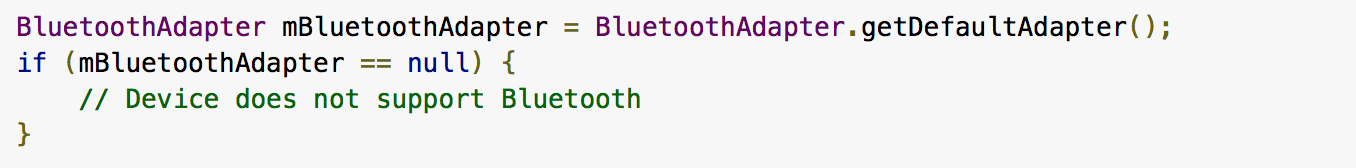
\includegraphics[scale=0.60]{bluetooth_enabled}
  	\caption{Trecho de código exemplificando a comunicação \textit{bluetooth}}
  	\label{img:bluetooth_enabled}
  	\end{figure}
  	
  	Para garantir que o dispositivo \textit{bluetooth} será adicionado apenas uma vez, será utilzado um trecho de código parecido com o da figura \ref{img:bluetooth_devices}, que garante que para um dispositivo ser adicionado ele, não deve estar presente na lista de dispositivos previamente adicionados.
  	
  	\graphicspath{{figuras/}}
  	\begin{figure}[h]
  	\centering
  	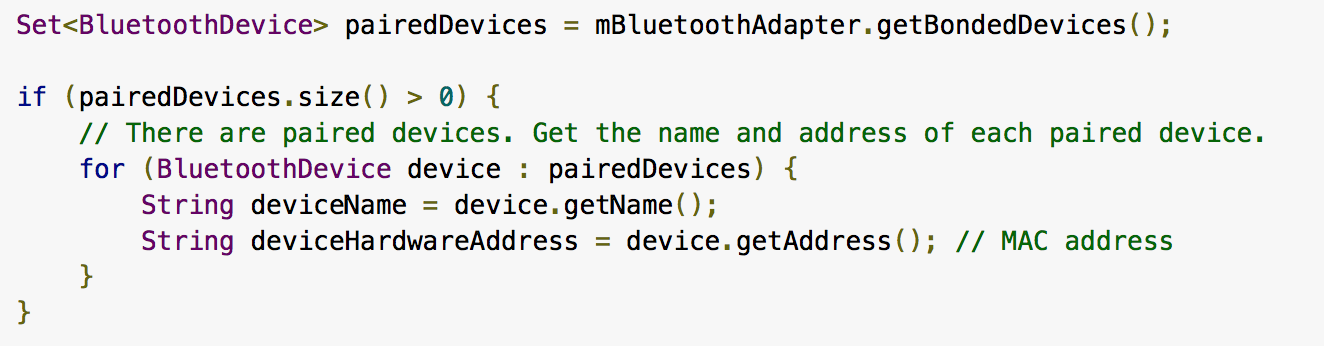
\includegraphics[scale=0.60]{bluetooth_paired_devices}
  	\caption{Trecho de Código que garante que um dispositivo será adicionado apenas uma vez}
  	\label{img:bluetooth_devices}
  	\end{figure}
  	
  	Para que seja feita a transferência de dados entre os dispositivos, o Google (empresa responsável pela documentação da plataforma android), dispõe um trecho de código que serve como guia para implementação desta funcionalidade. Na figura \ref{img:trecho1} é criada uma classe que define as constantes que serão utilizadas ao longo do código.
  	
  	\graphicspath{{figuras/}}
  	\begin{figure}[h!]
  	\centering
  	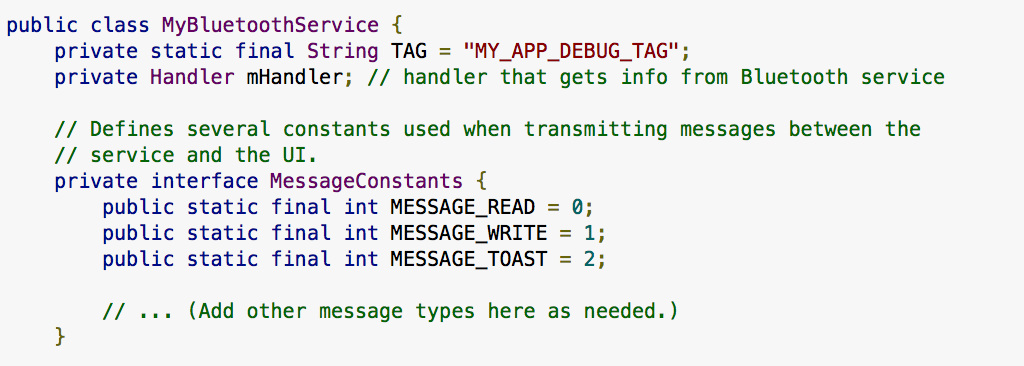
\includegraphics[scale=0.60]{classe_MyBluetoothService}
  	\caption{Neste trecho de código são definidas as constantes que serão utilizadas ao longo do código}
  	\label{img:trecho1}
  	\end{figure}
  
Na figura \ref{img:trecho2} é criada uma outra classe que é a classe que implementa a funcionalidade de troca de dados. Esta classe extende da classe Thread, seus atributos são do tipo \textit{BluetoothSocket}, \textit{InputStream}, \textit{OutputStream} e um \textit{array} de \textit{byte}.

\graphicspath{{figuras/}}
\begin{figure}[h!]
\centering
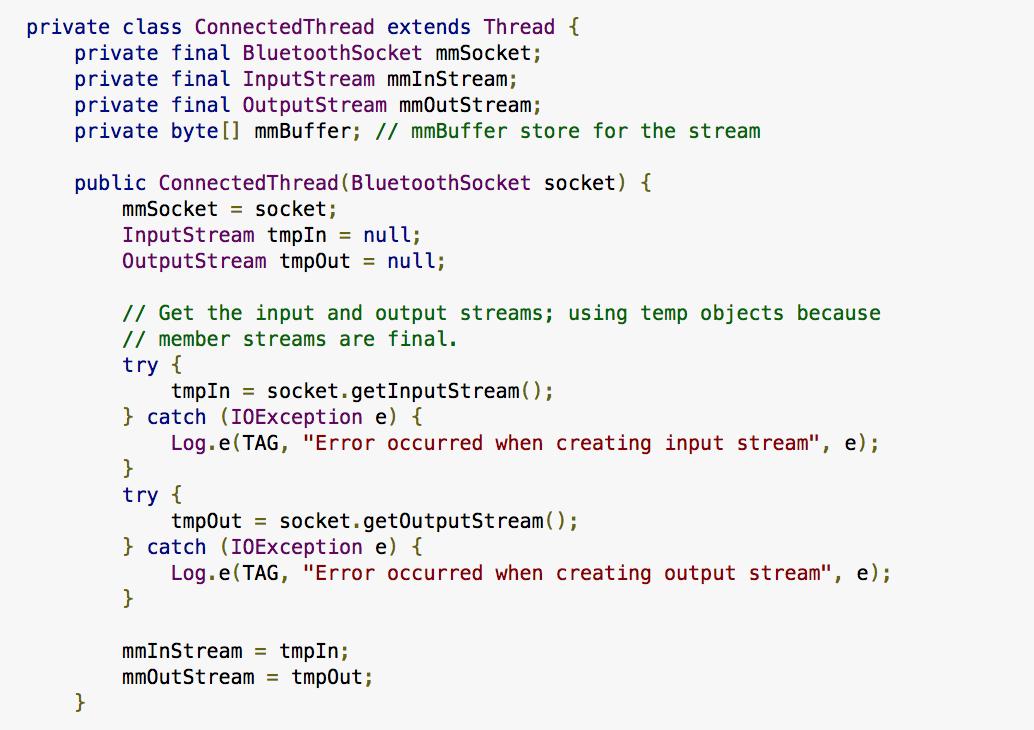
\includegraphics[scale=0.80]{classe_ConnectedThread}
\caption{Nesta classe são implementados os métodos responsáveis pelo funcionamento da troca de dados}
\label{img:trecho2}
\end{figure}

A figura \ref{img:trecho3} apresenta o método \textit{"run"} que funciona em segundo plano constantemente. Este método é responsável por ficar aguardando uma requisição do dispositivo.

\graphicspath{{figuras/}}
\begin{figure}[h!]
\centering
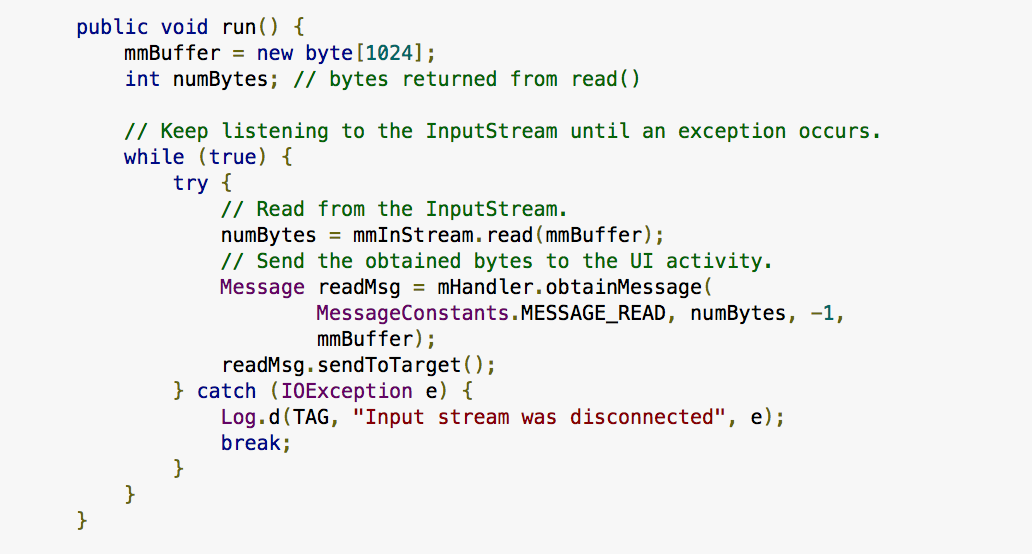
\includegraphics[scale=0.80]{run_method}
\caption{Implementação do método \textit{run} que é responsável por receber as informações do dispositivo \textit{bluetooth}}
\label{img:trecho3}
\end{figure}

O método \textit{"write"} é que faz a escrita dos dados que serão enviados para o dispositivo, como pode ser visto na figura \ref{img:trecho4}.

\graphicspath{{figuras/}}
\begin{figure}[h]
\centering
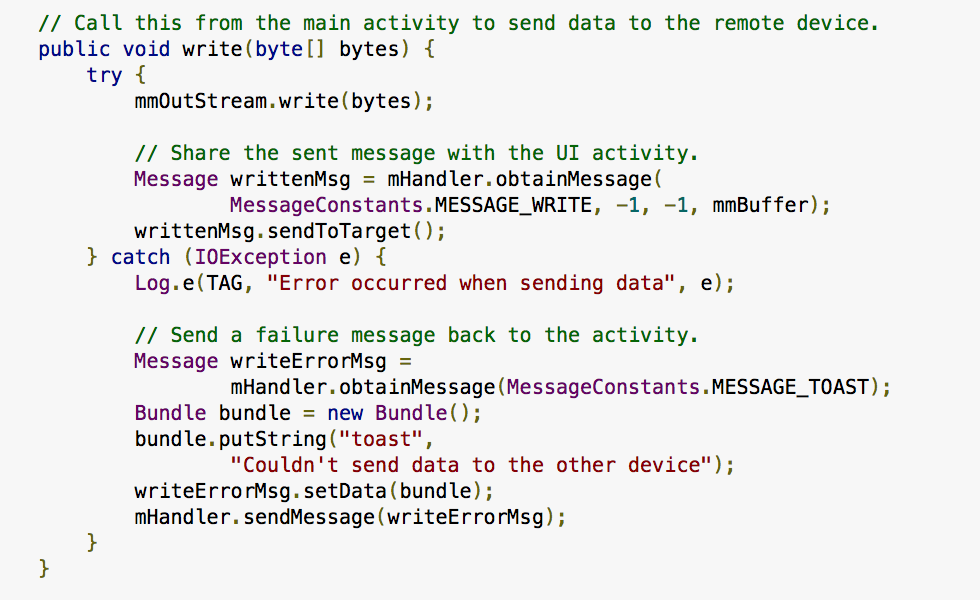
\includegraphics[scale=0.80]{write_method}
\caption{Implementação do método \textit{write} que é responsável por escrever os dados que serão enviados}
\label{img:trecho4}
\end{figure}

Por último, o método \textit{"cancel"} que encerra a conexão com o dispositivo pareado, como mostrado na figura \ref{img:trecho5}

\graphicspath{{figuras/}}
  \begin{figure}[h]
  \centering
  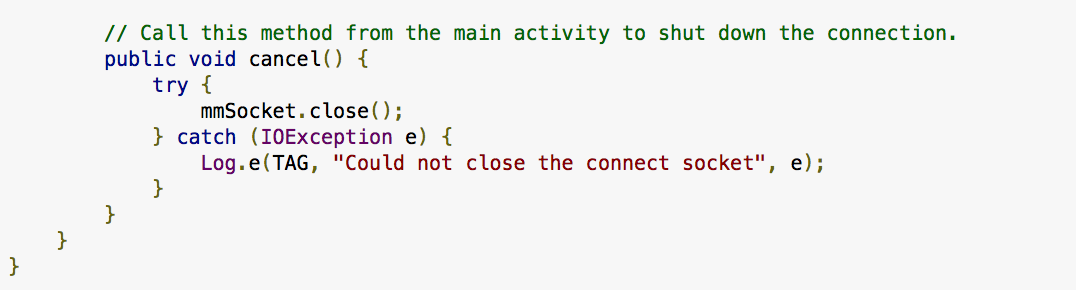
\includegraphics[scale=0.80]{cancel_method}
  \caption{Método \textit{"cancel"} que encerra a conexão com o dispositivo}
  \label{img:trecho5}
  \end{figure}  
  
  \section{Eletroeletrônica}
  	\subsection{Acionamento do Motor}
  
 	 \subsection{Sistema de Controle}
  
  \section{Alimentação}
  A bicicleta elétrica utilizará dois sistemas de alimentação, que serão:
  \begin{itemize}
  	\item Banco de baterias para alimentar o motor elétrico;
  	\item Dínamo para carregar uma bateria que alimentará os componentes eletrônicos e todo o sistema de iluminação do GPS. 
  \end{itemize}
  
	O sistema de navegação será alimentado por um sistema separado do motor elétrico como forma de garantia de suprimento de energia para esse sistema. Caso a bateria descarregue no meio do percurso, o dínamo será capaz de carregá-la enquanto o ciclista pedala a bicicleta, garantindo que o mesmo continuará com o sistema de iluminação que lhe indicará a rota desejada.
	
	\subsection{Motor Elétrico}
	
	
	\subsection{Dínamo}
	Gerador elétrico é uma máquina capaz de converter energia mecânica em energia elétrica, baseado no princípio físico de indução magnética \cite{maximo}. O dínamo é um tipo de gerador elétrico e foi primeiramente utilizado em bicicletas em 1896, patenteado por Alfred Rodriguez. Um dínamo típico utilizado em bicicletas pode ser visto na Figura \ref{img:dinamo_bicicleta}.
	
	\graphicspath{{figuras/}}
	\begin{figure}[h!]
	\centering
	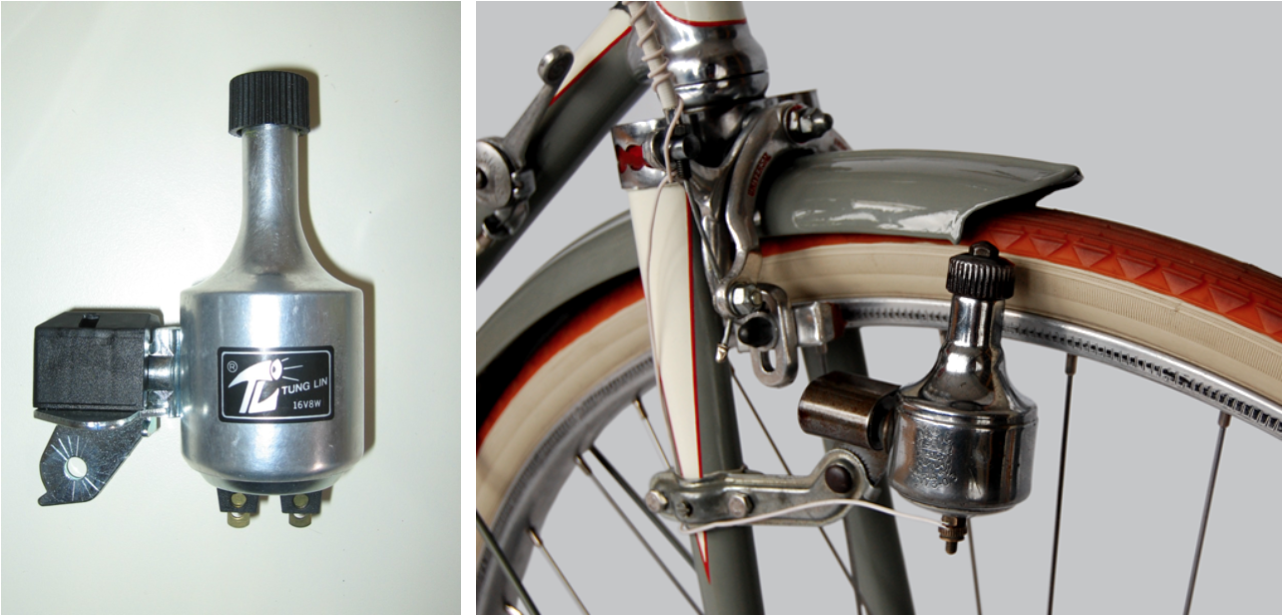
\includegraphics[scale=0.60]{dinamo_bicicleta}
	\caption{Dínamo de Bicicleta}
	\label{img:dinamo_bicicleta}
	\end{figure}
	
Acoplado à roda da bicicleta, o dínamo utiliza a energia cinética de rotação da roda girando um íma que excitará as bobinas circundantes gerando corrente elétrica, que será retificada e irá carregar a bateria por meio de cabos. A bateria irá, então, alimentar os componentes eletrônicos como o microcontrolador e as placas de LED.

A potência mecânica é dada pelo produto do torque () e da velocidade angular () da roda da bicicleta, como visto na Figura \ref{img:potencia_mecanica}. 

\graphicspath{{figuras/}}
\begin{figure}[h!]
\centering
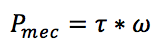
\includegraphics[scale=1.0]{potencia_mecanica}
\caption{Fórmula de potência mecânica}
\label{img:potencia_mecanica}
\end{figure}

Sendo que o torque é dado pela equação da figura \ref{img:torque}, onde r é o raio da roda

\graphicspath{{figuras/}}
\begin{figure}[h!]
\centering
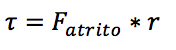
\includegraphics[scale=1.0]{torque}
\caption{Fórmula para cálculo do torque}
\label{img:torque}
\end{figure}


As velocidades serão medidas experimentalmente com o uso de um tacômetro e a tensão e corrente de saída do dínamo com um multímetro.
  
\subsection{Bateria}
	Baterias são dispositivos capazes de converter energia química em energia elétrica através de reações de oxirredução. Ao ligar dois componentes químicos de polos opostos, anodo e catodo, uma diferença de potencial é gerada e elétrons migram do polo negativo, anodo, para o polo positivo, catodo, gerando, assim, uma corrente elétrica. Algumas também são capazes de fazer o processo inverso, convertendo energia elétrica em energia química. Dessa forma, as baterias são usadas como uma fonte de energia elétrica e como armazenamento dessa energia \cite{varela}.
	
	Os tipos de bateria mais utilizadas são: chumbo-ácido, níquel-metal hidreto e íon-lítio.
	
	\begin{itemize}
		\item \textbf{Chumbo-Ácido}: São as baterias com maior maturação no mercado por serem utilizadas há mais tempo, apresentam baixo custo e confiabilidade, sendo muito utilizadas para partidas de motores de automóveis, iluminação, ignição e tração. Sua densidade de energia e energia específica, porém, são a de menor valor \cite{bezerra}.
	\item \textbf{Íon-Lítio}:  São baterias mais leves, com alta densidade de energia, maior eficiência energética que as demais e elevado número de ciclos de vida. O custo é ainda muito alto e a tolerância a sobrecarga é baixa correndo riscos de danificação \cite{bezerra}. São muito utilizadas em aparelhos eletrônicos como celulares e laptops.
	\end{itemize}
	
	A capacidade de uma bateria é dada pela equação da figura \ref{img:calculo_bateria}
	
	\graphicspath{{figuras/}}
	\begin{figure}[h!]
	\centering
	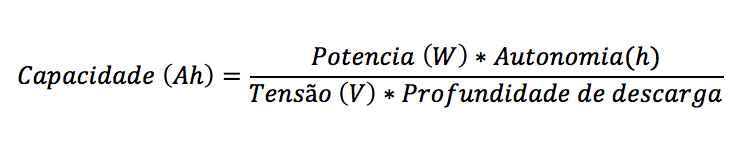
\includegraphics[scale=1.0]{capacidade_bateria}
	\caption{Fórmula para cálculo da bateria}
	\label{img:formula_capacidade}
	\end{figure}
	

	SANCHES \cite{daanalise} coletou informações sobre rotas cíclicas mais escolhidas por ciclistas quando usando GPS. Em seus resultados, os percursos mais longos feitos duravam, em média, 20 minutos e os participantes da pesquisa faziam, em média, 2,5 viagens por dia. Os percursos totais, por dia, para cada ciclista, duram, em média, 50 minutos. Para dimensionar a bateria, portanto, considera-se o motor trabalhando em máxima potência e o tempo de autonomia de 1h.
	
	\graphicspath{{figuras/}}
	\begin{figure}[h!]
	\centering
	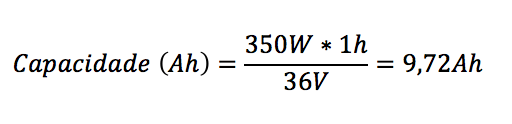
\includegraphics[scale=1.0]{calculo_capacidade}
	\caption{Cálculo da bateria a ser utilizada}
	\label{img:calculo_bateria}
	\end{figure}
	
	Portanto, para alimentar o motor, serão utilizadas três baterias chumbo-ácido de 12V cada, ligadas em série, com capacidade de 10Ah. A escolha desse tipo de bateria foi escolhida devido ao menor custo e maior disponibilidade por ser uma tecnologia mais madura para aplicações automotivas.

	A demanda de corrente típica de cada componente eletrônico segue listado abaixo:
	
	\begin{itemize}
		\item \textbf{Microcontrolador}: 40mA por pino. Um arduíno possui 14 pinos, supondo que sejam usadas todas as entradas, o arduíno demandará 700mA.
		\item \textbf{Microprocessador}: 50A.
		\item \textbf{LED}: 20mA cada.

	\end{itemize}

Os componentes demandam uma corrente de 800 a 900mA. Será utilizada uma bateria de 12V e 1,3Ah que o grupo já possui.

  
  \section{Estrutura}
  Este projeto visa a construção de uma bicicleta elétrica capaz de seguir uma rota pré-determinada via gps. Porém, há a necessidade de se projetar com a devida atenção toda a estrutura da bicicleta de modo que os demais componentes sejam devidamente adaptados de forma ergonômica, em outras palavras, maximizar a segurança e eficiência da interação máquina e ser humano.
Foram levados em consideração vários fatores, como o material, a estabilidade, conforto e custo-benefício para a escolha e dimensionamento da estrutura.O quadro da bicicleta guardará os motores, baterias e demais componentes eletroeletrônicos de forma segura e organizada. Haverá também, um painel bastante intuitivo que auxiliará o usuário em sua rota como: indicação da bateria restante, distância percorrida e distância restante.
	
	\subsection{Materiais}
	Dentre os materiais que compõem o quadro da bicicleta, foi se escolhido o alumínio, por se tratar de um material leve, barato, com ponto de fusão suficientemente seguro para ser integrado com os componentes eletroeletrônicos além da pouca oxidação sofrida. Outros materiais que foram pesquisados com a finalidade de implementação, foram o aço, porém possui um peso elevado se comparado ao alumínio, e está sujeito a oxidação, apesar do baixo preço. Fibra de carbono, possui um baixo peso, porém um alto custo e uma grande dificuldade na parte de manutenção e conserto.
	
	\subsection{Ergonomia}
	Atualmente no mercado brasileiro as bicicletas mais vendidas são as Mountain Bike, comumente apelidadas de MTB. Isso se deve a sua versatilidade que permite ser utilizada em qualquer terreno. Elas geralmente são encontradas nos tamanho de quadro 17, 18 e 19”. Os dois primeiros tipos são indicados para pessoas entre 1,68 e 1,78 metros de altura enquanto a última atende a faixa de 1,78 e 1,85 metros. 
Segundo a pesquisa de orçamentos familiares realizada pelo IBGE entre 2008 e 2009, a estatura média da mulher e do homem brasileiro adulto são, respectivamente, 1,71 e 1,60 metros. Associando esse dado com os tamanhos de quadros mais comuns do mercado optou-se por utilizar como base para o projeto um quadro de 17”.  
As análises ergonômicas serão realizadas com o auxílio do software CATIA V5 utilizando sua base de dados referente ao estudo de percentil do norte americano. Para o problema apresentado serão adotadas as medidas dos homens de percentil entre 13 e 65, e para mulheres entre 79 e 99, ambos norte americanos.

	\subsection{Design}

	O \textit{design} da bicicleta é apresentado na figura \ref{img:dimensoes}, onde é possível ver as dimensões da bicicleta a ser produzida.	
	
	\graphicspath{{figuras/}}
	\begin{figure}[h!]
	\centering
	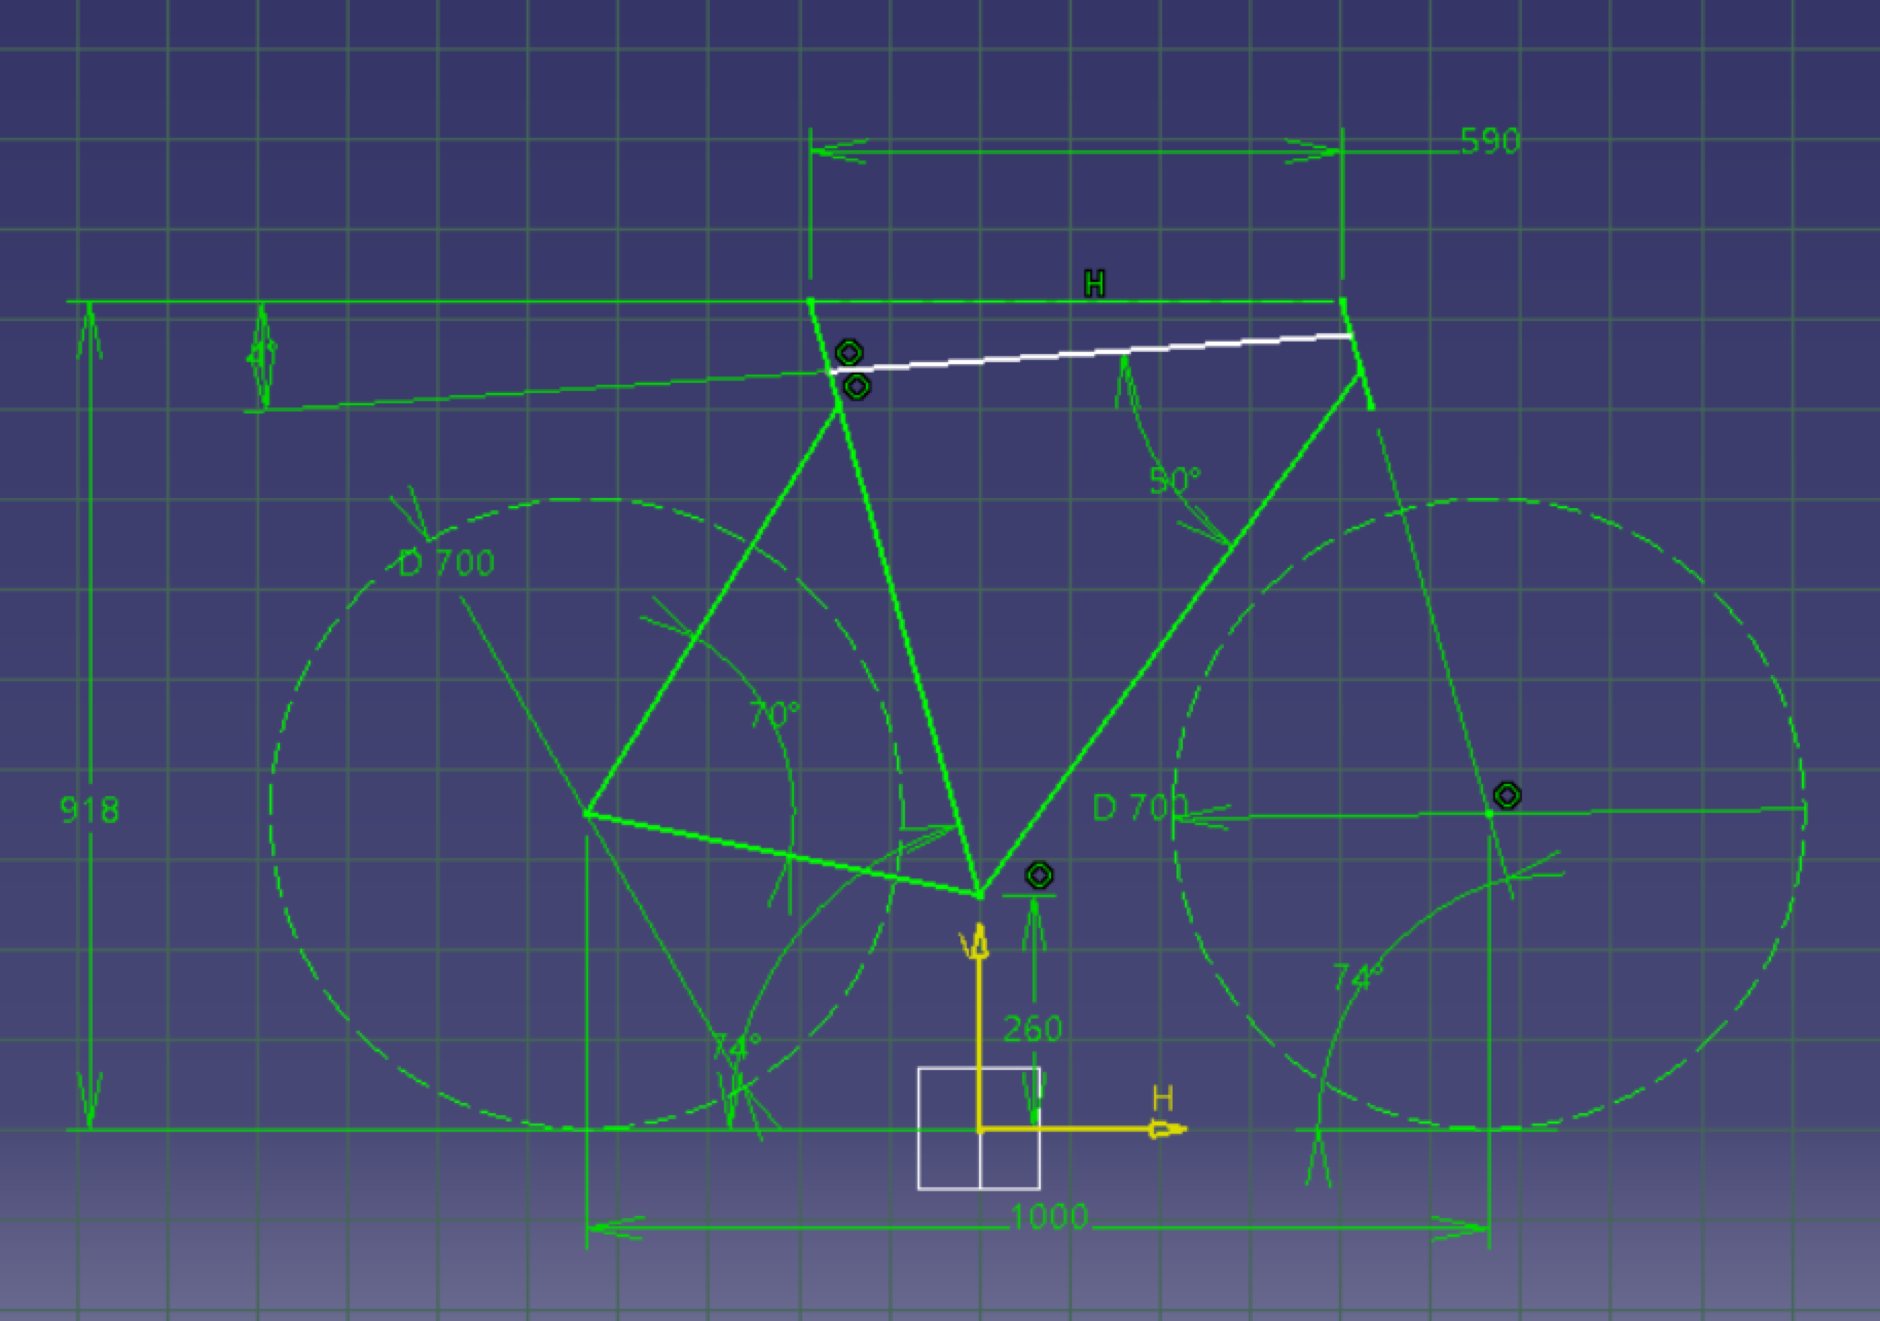
\includegraphics[scale=0.80]{dimensoes.png}
	\caption{Dimensões}
	\label{img:dimensoes}
	\end{figure}


	\subsection{Estabilidade}
	O centro de massa da bicicleta sem os componentes se concentrou em 0,6m no eixo x e 0,5m no eixo y, as forças normais nos pneus traseiros e dianteiros foram de,respectivamente: 24,525N e 73,575N, enquanto as forças de fricção(atrito)  nos pneus traseiros e dianteiros de,respectivamente: 14,96N e 44,88N. As figuras \ref{img:esq_forca_sem_frenagem}, \ref{img:esq_forca_com_frenagem_suave} e \ref{img:esq_forca_com_frenagem_brusca} apresentam três esquemáticos demonstrando a aplicação da força sobre a bicicleta em três momentos distintos. 

\graphicspath{{figuras/}}
\begin{figure}[h!]
\centering
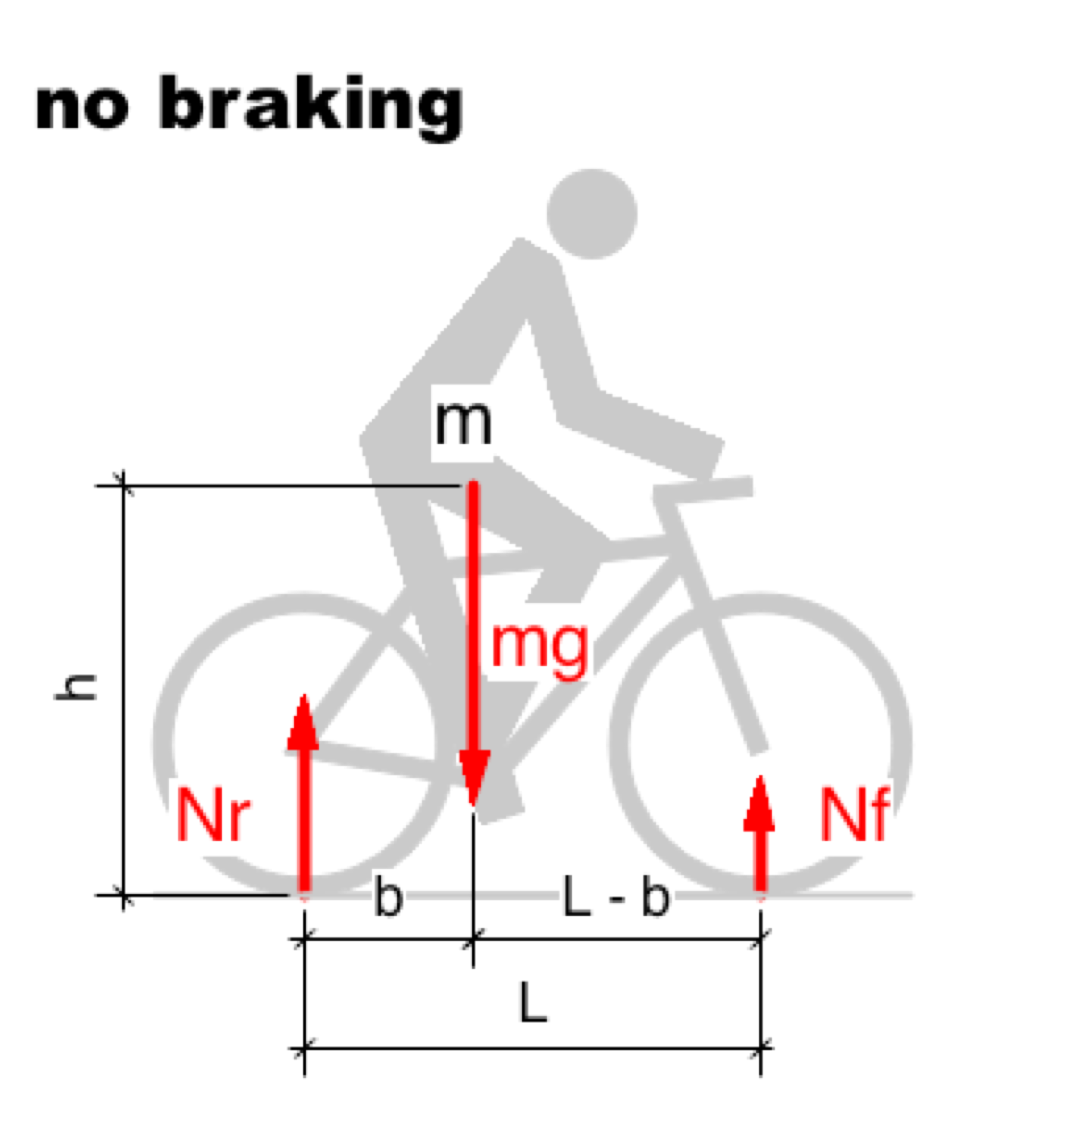
\includegraphics[scale=0.80]{esq_forca_sem_frenagem.png}
\caption{Esquemático de força sem frenagem}
\label{img:esq_forca_sem_frenagem}
\end{figure}

\graphicspath{{figuras/}}
\begin{figure}[h!]
\centering
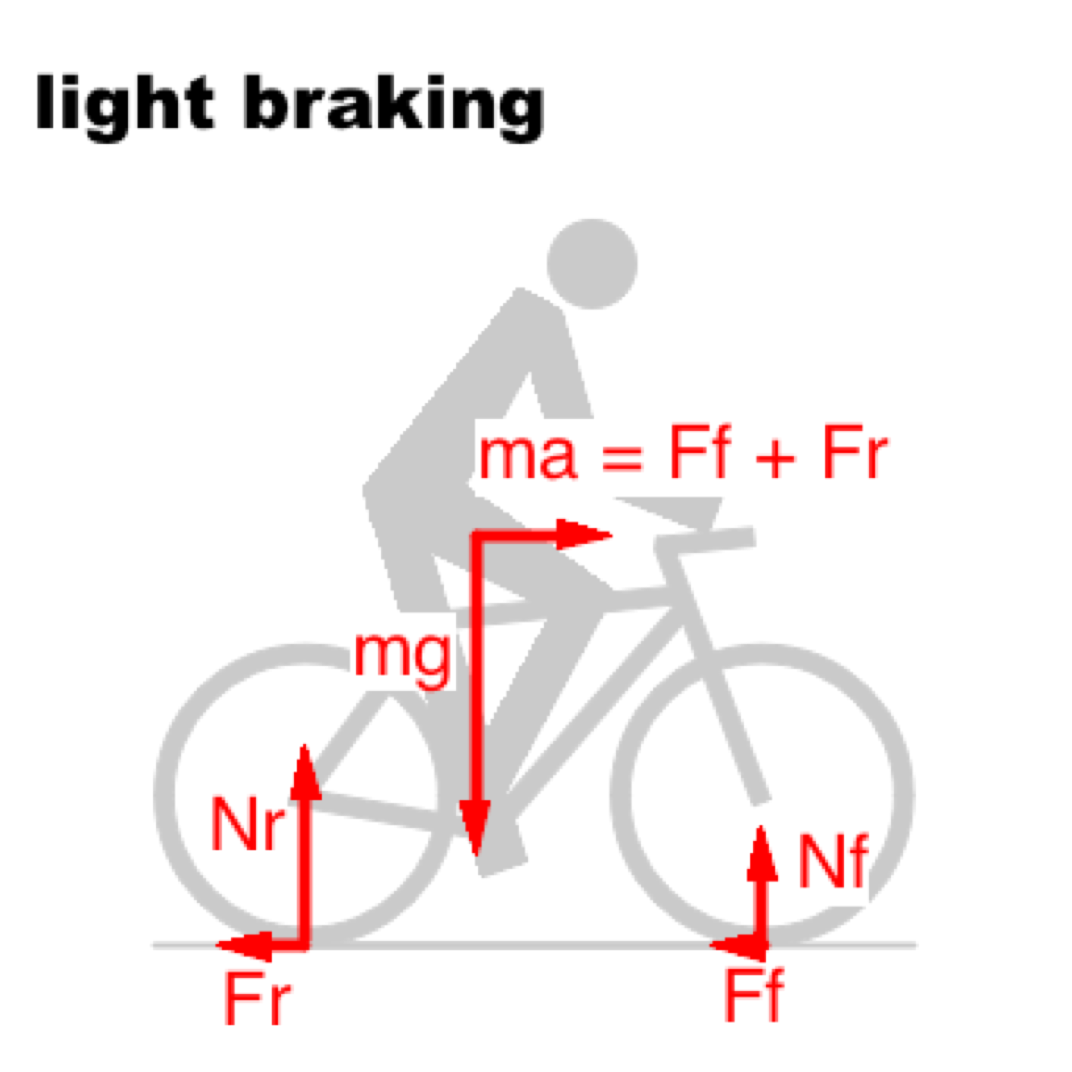
\includegraphics[scale=0.80]{esq_forca_com_frenagem_suave.png}
\caption{Esquemático de força com frenagem suave}
\label{img:esq_forca_com_frenagem_suave}
\end{figure}

\graphicspath{{figuras/}}
\begin{figure}[h!]
\centering
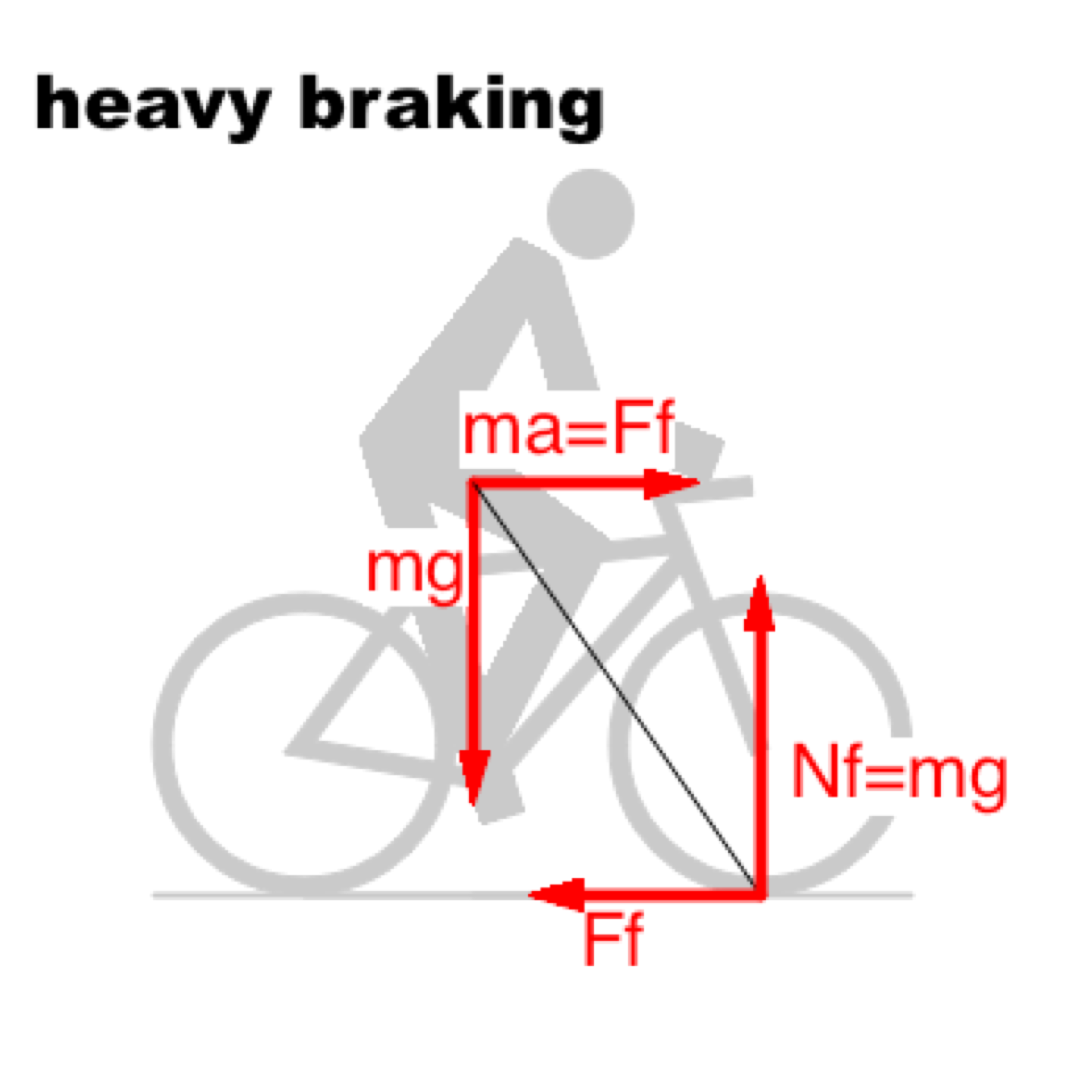
\includegraphics[scale=0.80]{esq_forca_com_frenagem_brusca.png}
\caption{Esquemático de forca com frenagem brusca}
\label{img:esq_forca_com_frenagem_brusca}
\end{figure}


	\subsection{Análises}
	Foram feitas algumas análises em um quadro de 17 com ajuda dos softwares CATIA v5 e Ansys R17.0 no intuito de levantar questões sobre requisitos e melhorias que deverão estar presentes na estrutura.
	
	\subsection{Estática}
	As figuras \ref{img:deformacao_total}, \ref{img:equivalente_de_von_mises}, \ref{img:modo_de_vibracao}, \ref{img:modo_de_vibracao2}, \ref{img:modo_de_vibracao3}, \ref{img:modo_de_vibracao4}, \ref{img:modo_de_vibracao5} e \ref{img:modo_de_vibracao 6} apresentam alguns graus de deformação à qual a bicicleta pode ser submetida. 	
	
\graphicspath{{figuras/}}
	\begin{figure}[h!]
	\centering
	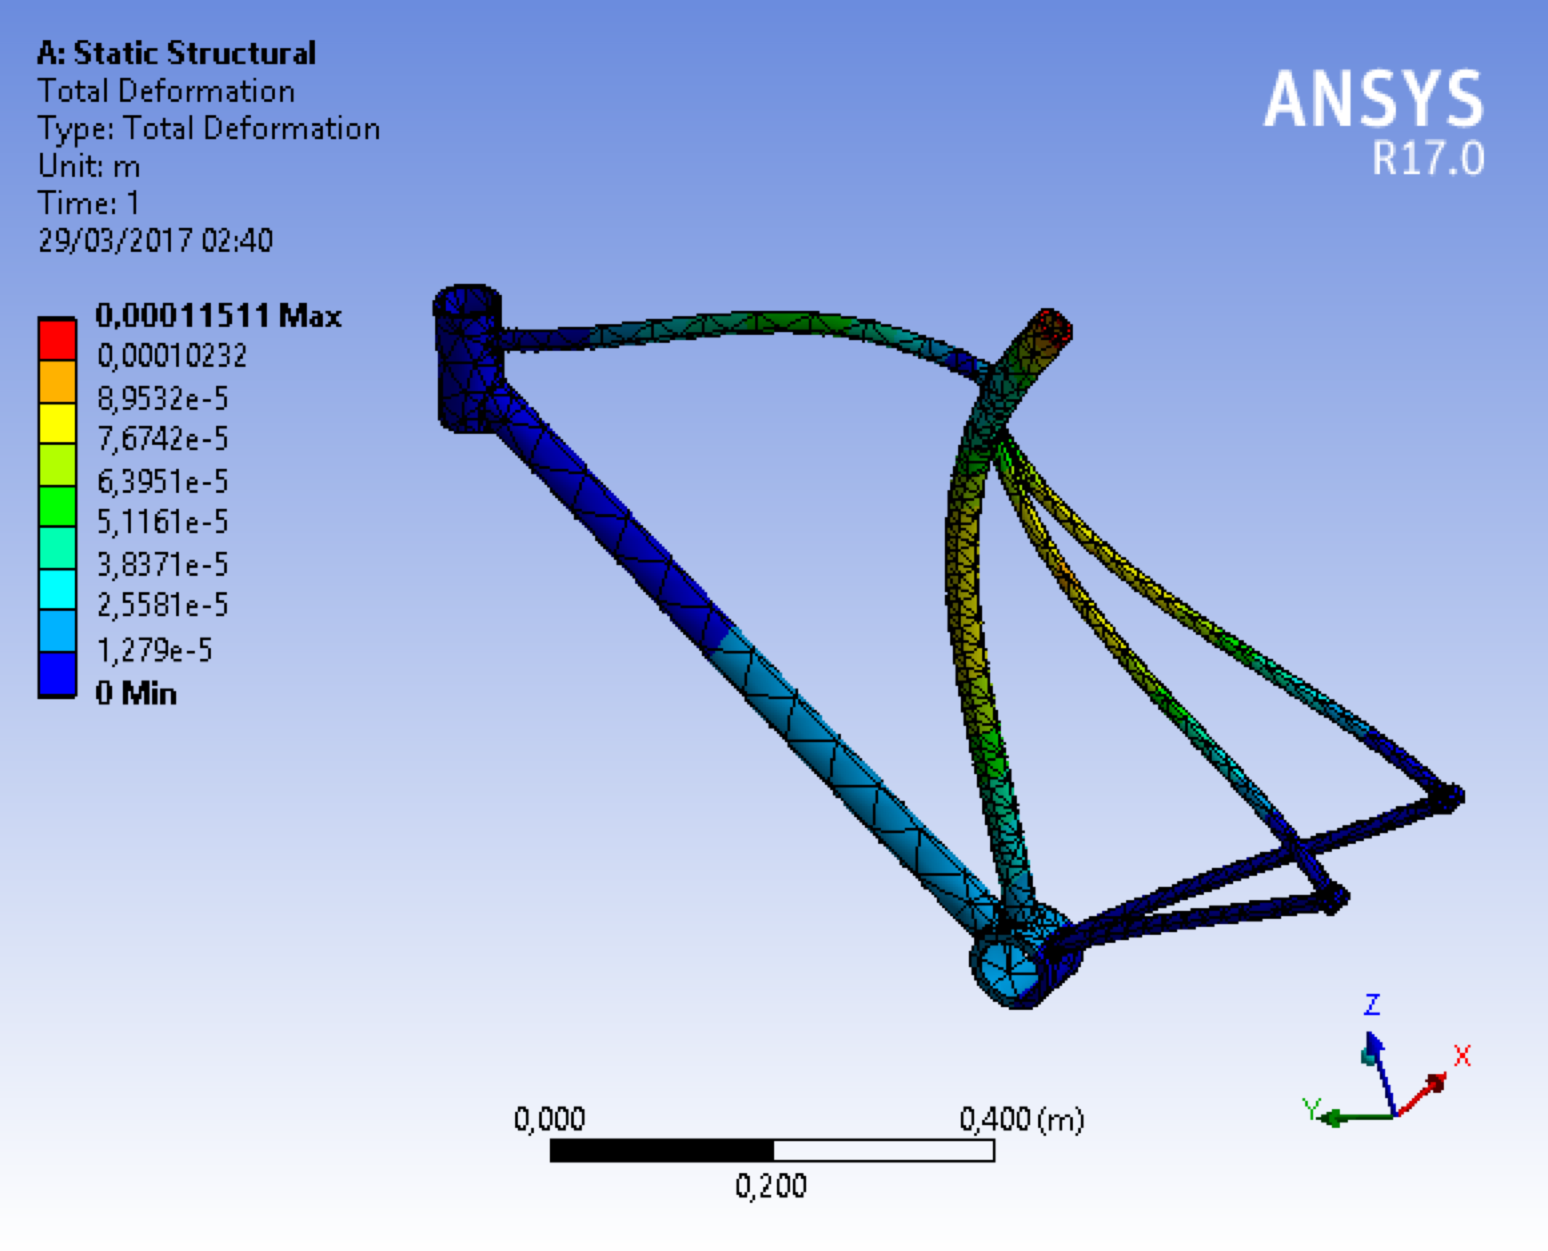
\includegraphics[scale=0.80]{deformacao_total.png}
	\caption{Deformacao total}
	\label{img:deformacao_total}
	\end{figure}	
	
\graphicspath{{figuras/}}
	\begin{figure}[h!]
	\centering
	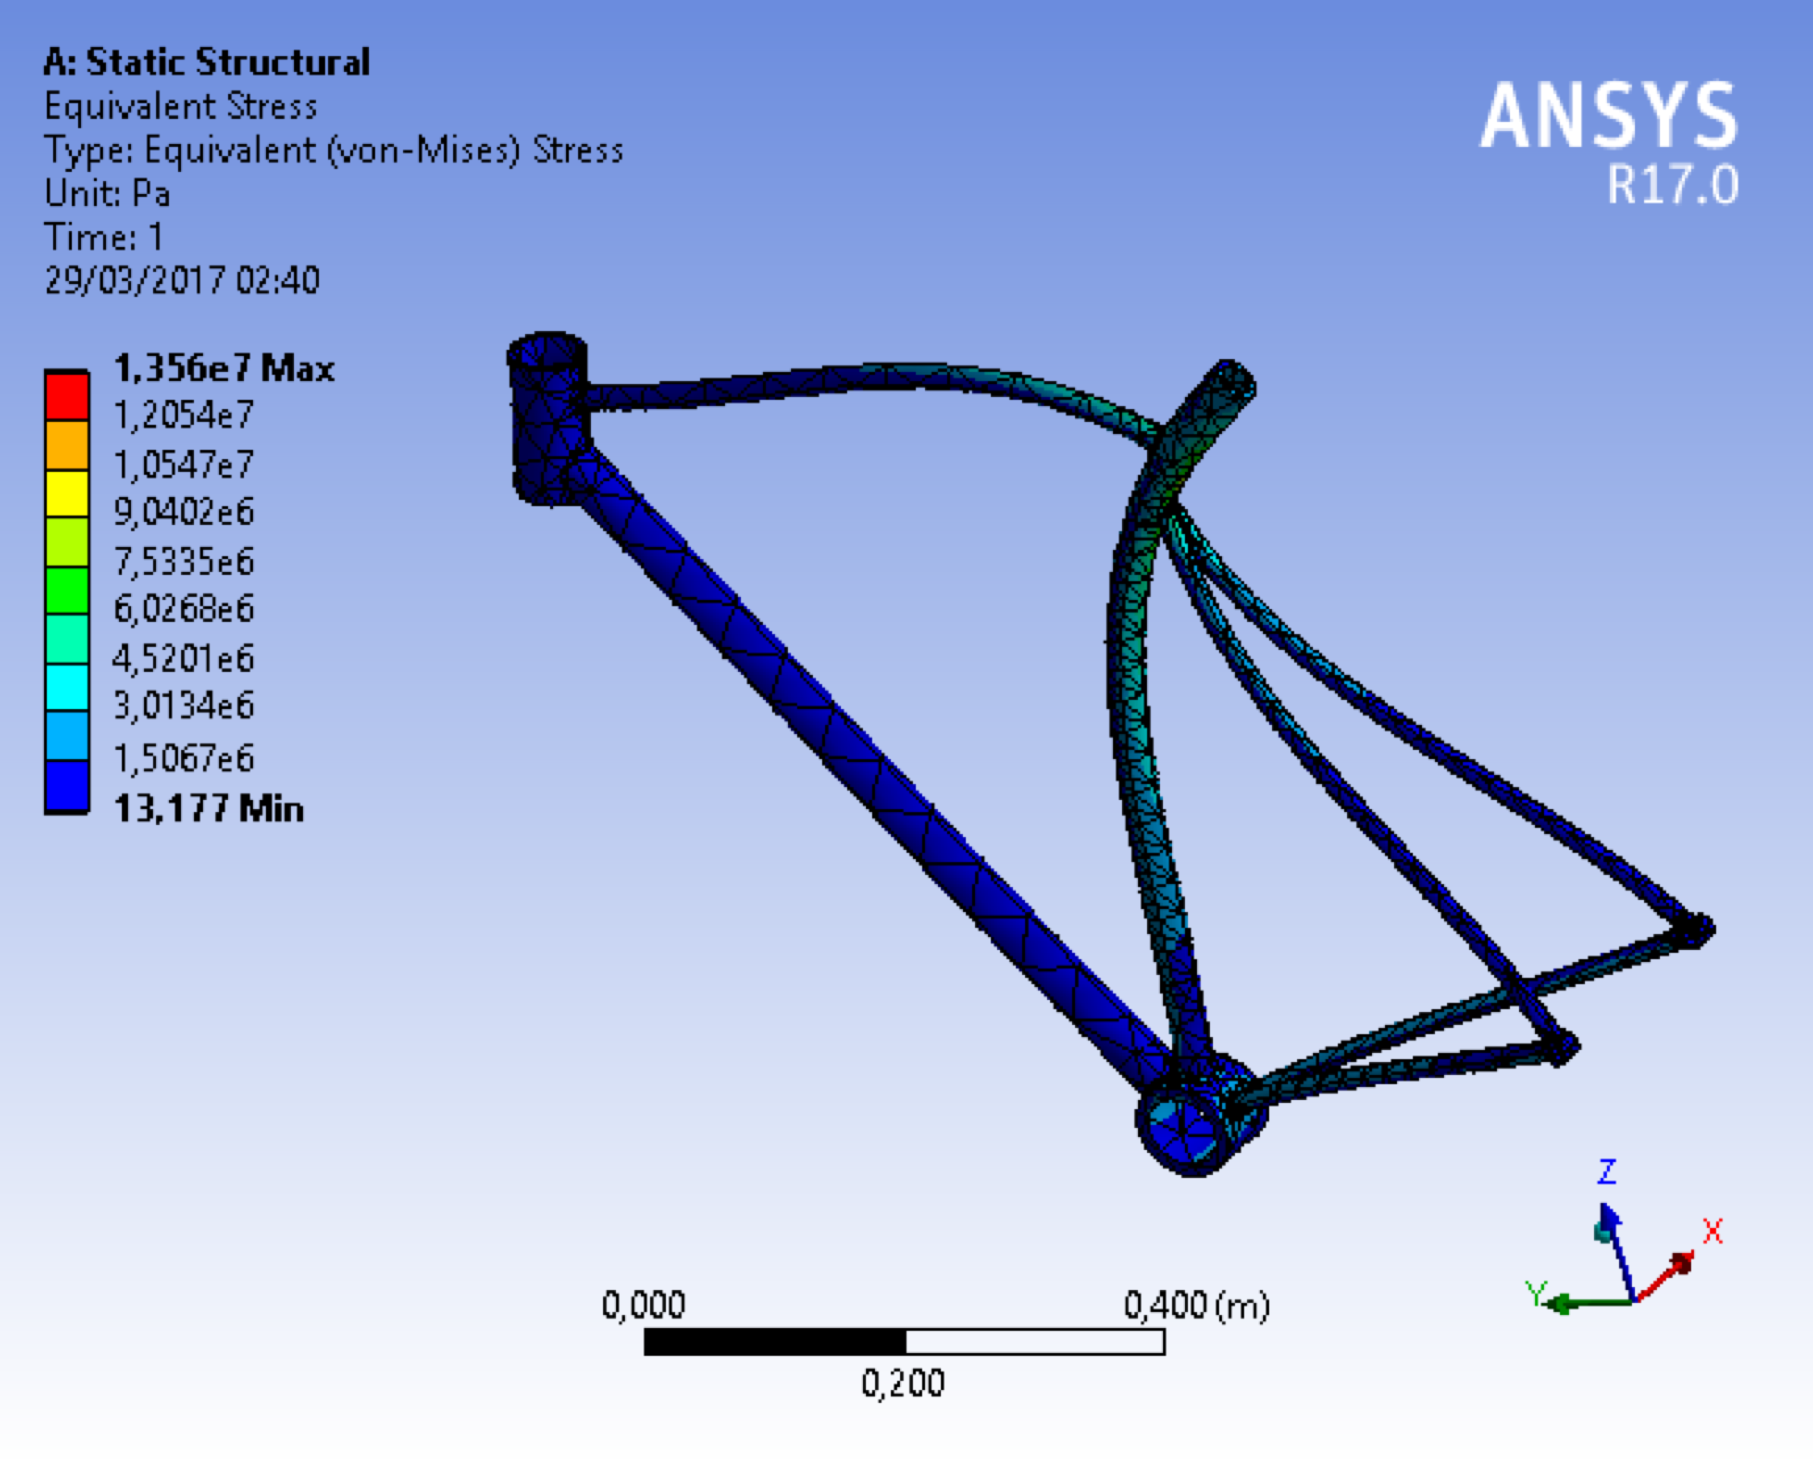
\includegraphics[scale=0.80]{equivalente_de_von_mises.png}
	\caption{Equivalente de von Mises}
	\label{img:equivalente_de_von_mises}
	\end{figure}	
	
\graphicspath{{figuras/}}
	\begin{figure}[h!]
	\centering
	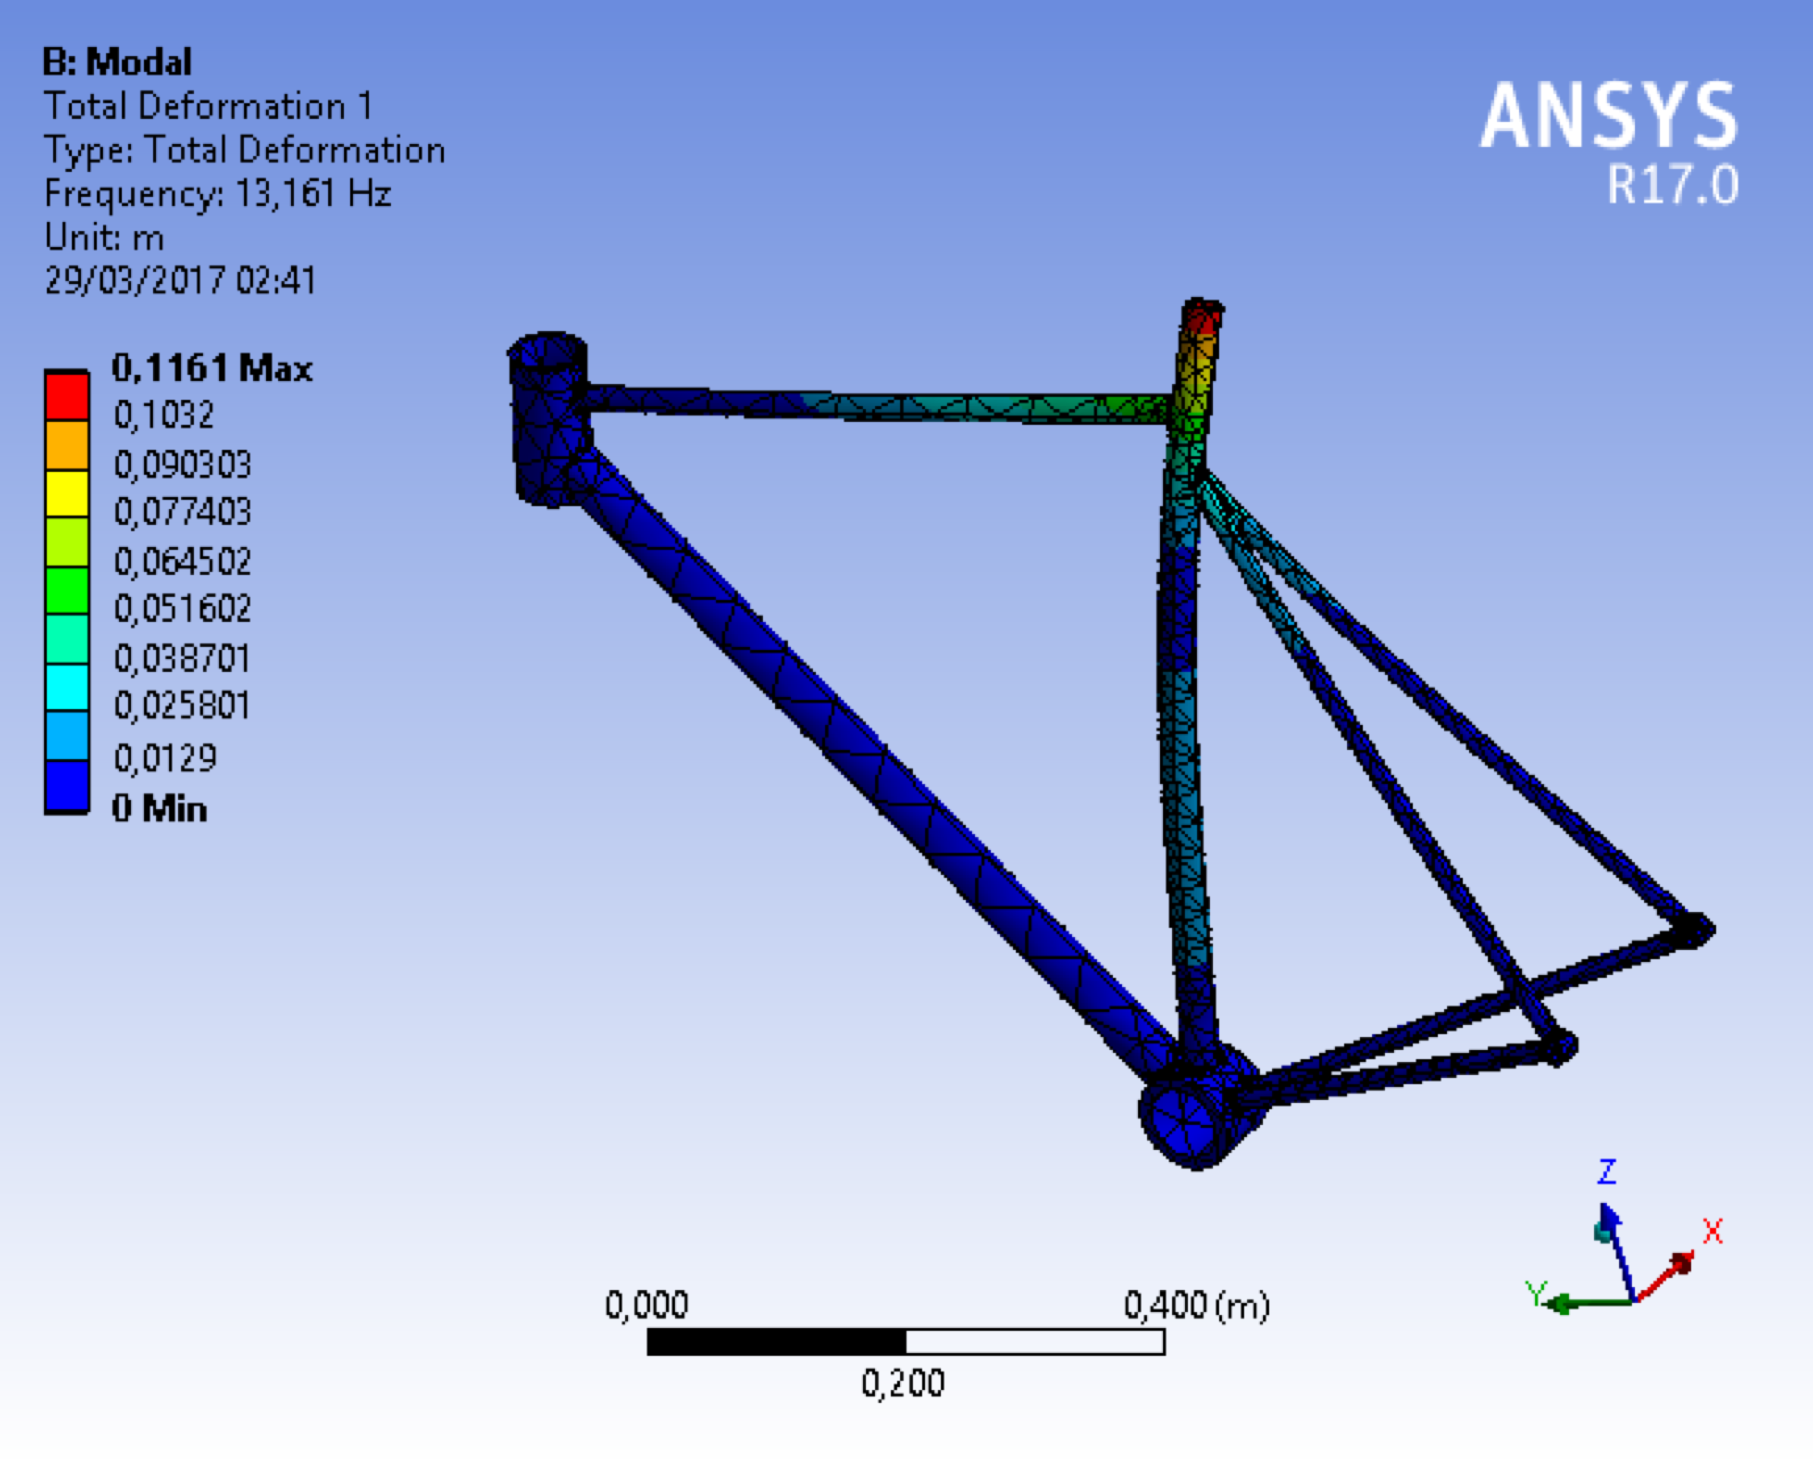
\includegraphics[scale=0.80]{modo_de_vibracao.png}
	\caption{Modo de vibracao}
	\label{img:modo_de_vibracao}
	\end{figure}	
	
\graphicspath{{figuras/}}
	\begin{figure}[h!]
	\centering
	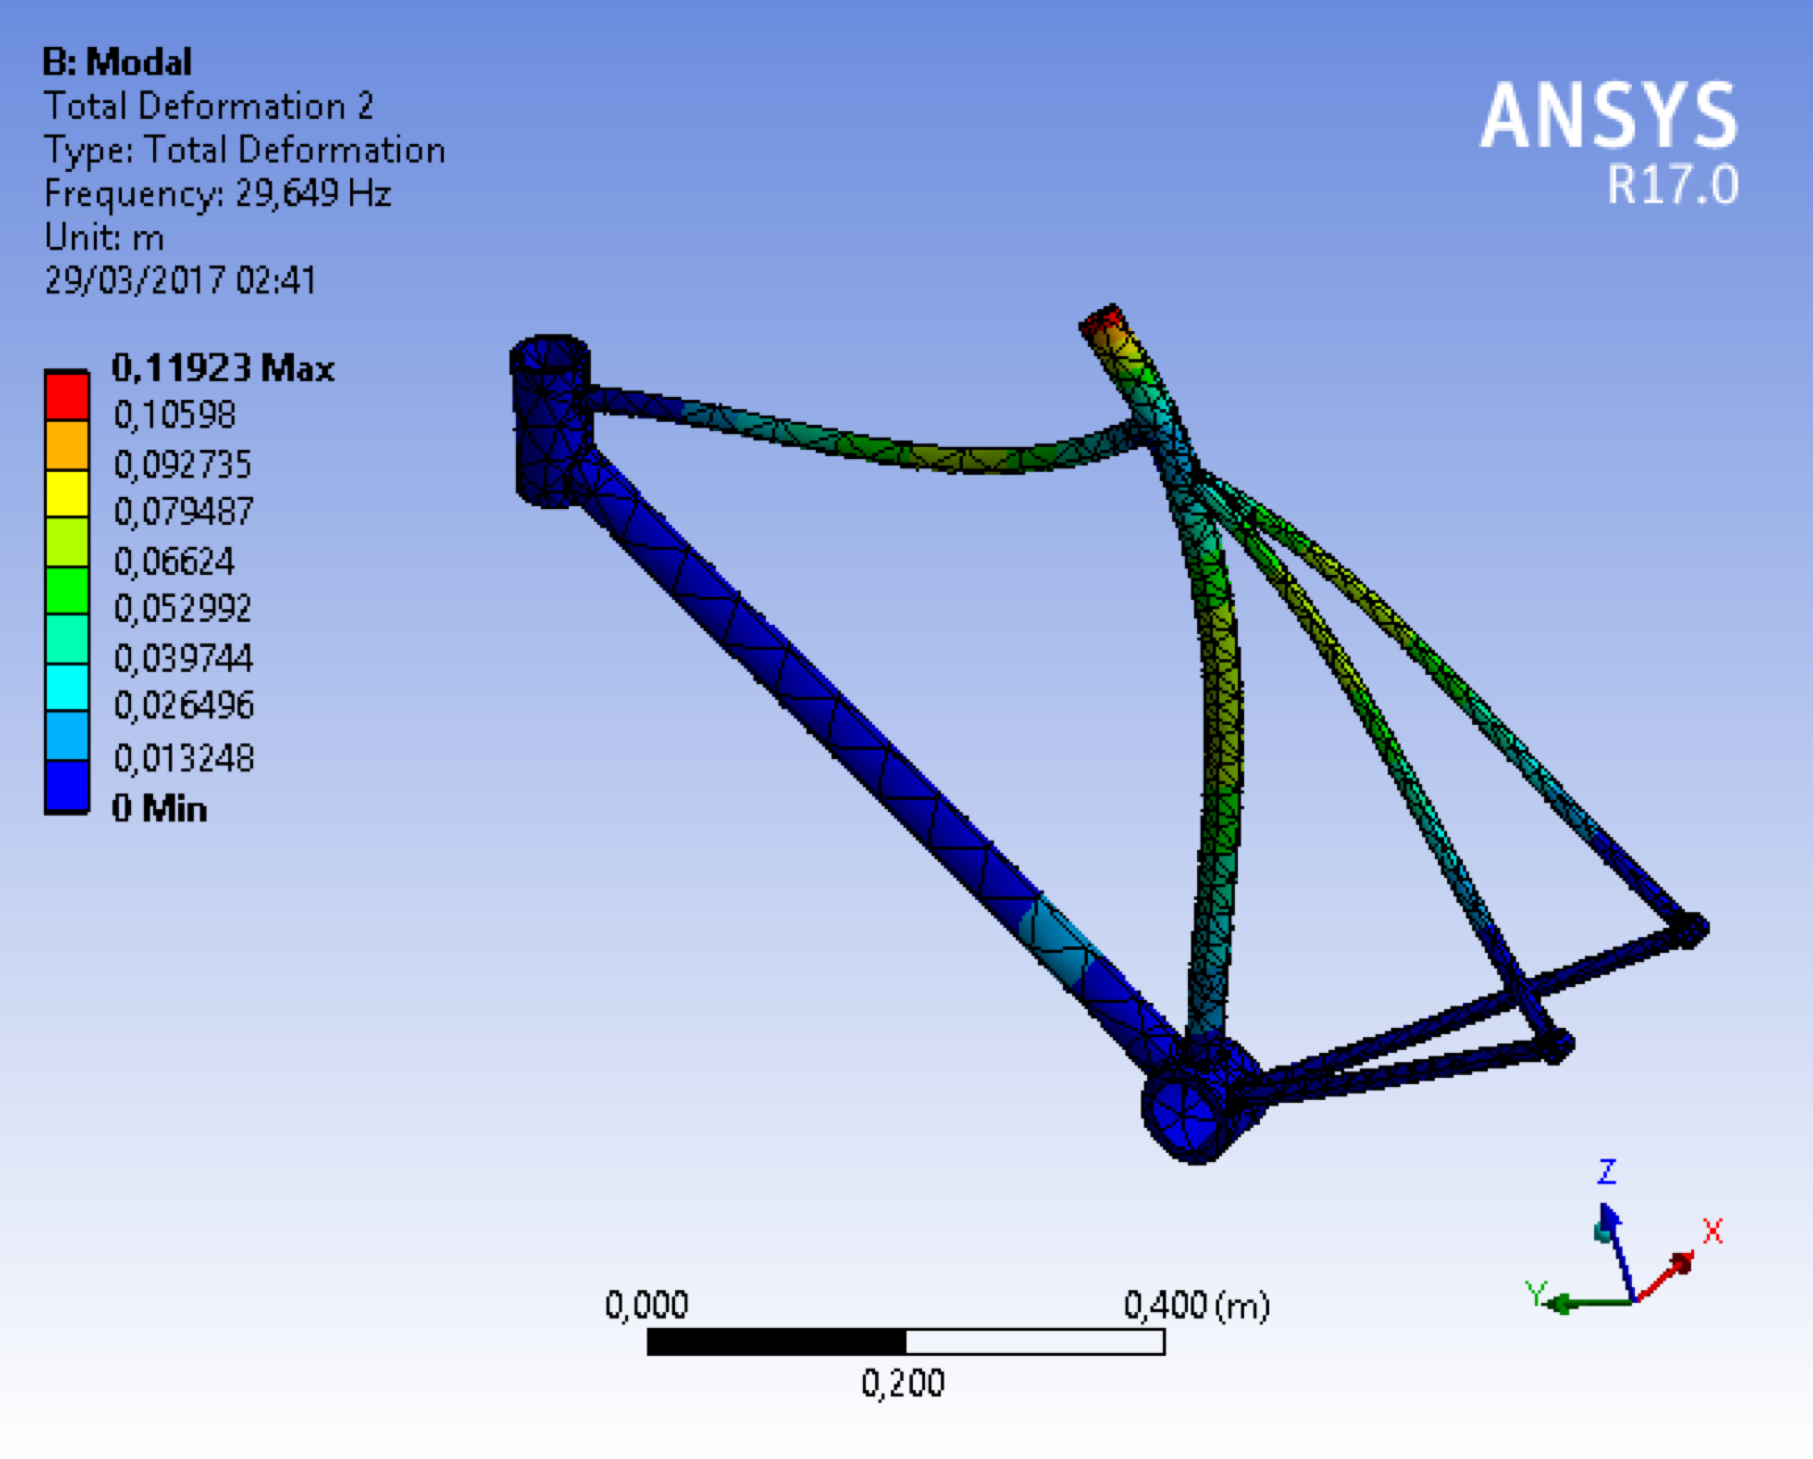
\includegraphics[scale=0.80]{modo_de_vibracao_2.png}
	\caption{Modo de vibracao 2}
	\label{img:modo_de_vibracao2}
	\end{figure}	
	
\graphicspath{{figuras/}}
	\begin{figure}[h!]
	\centering
	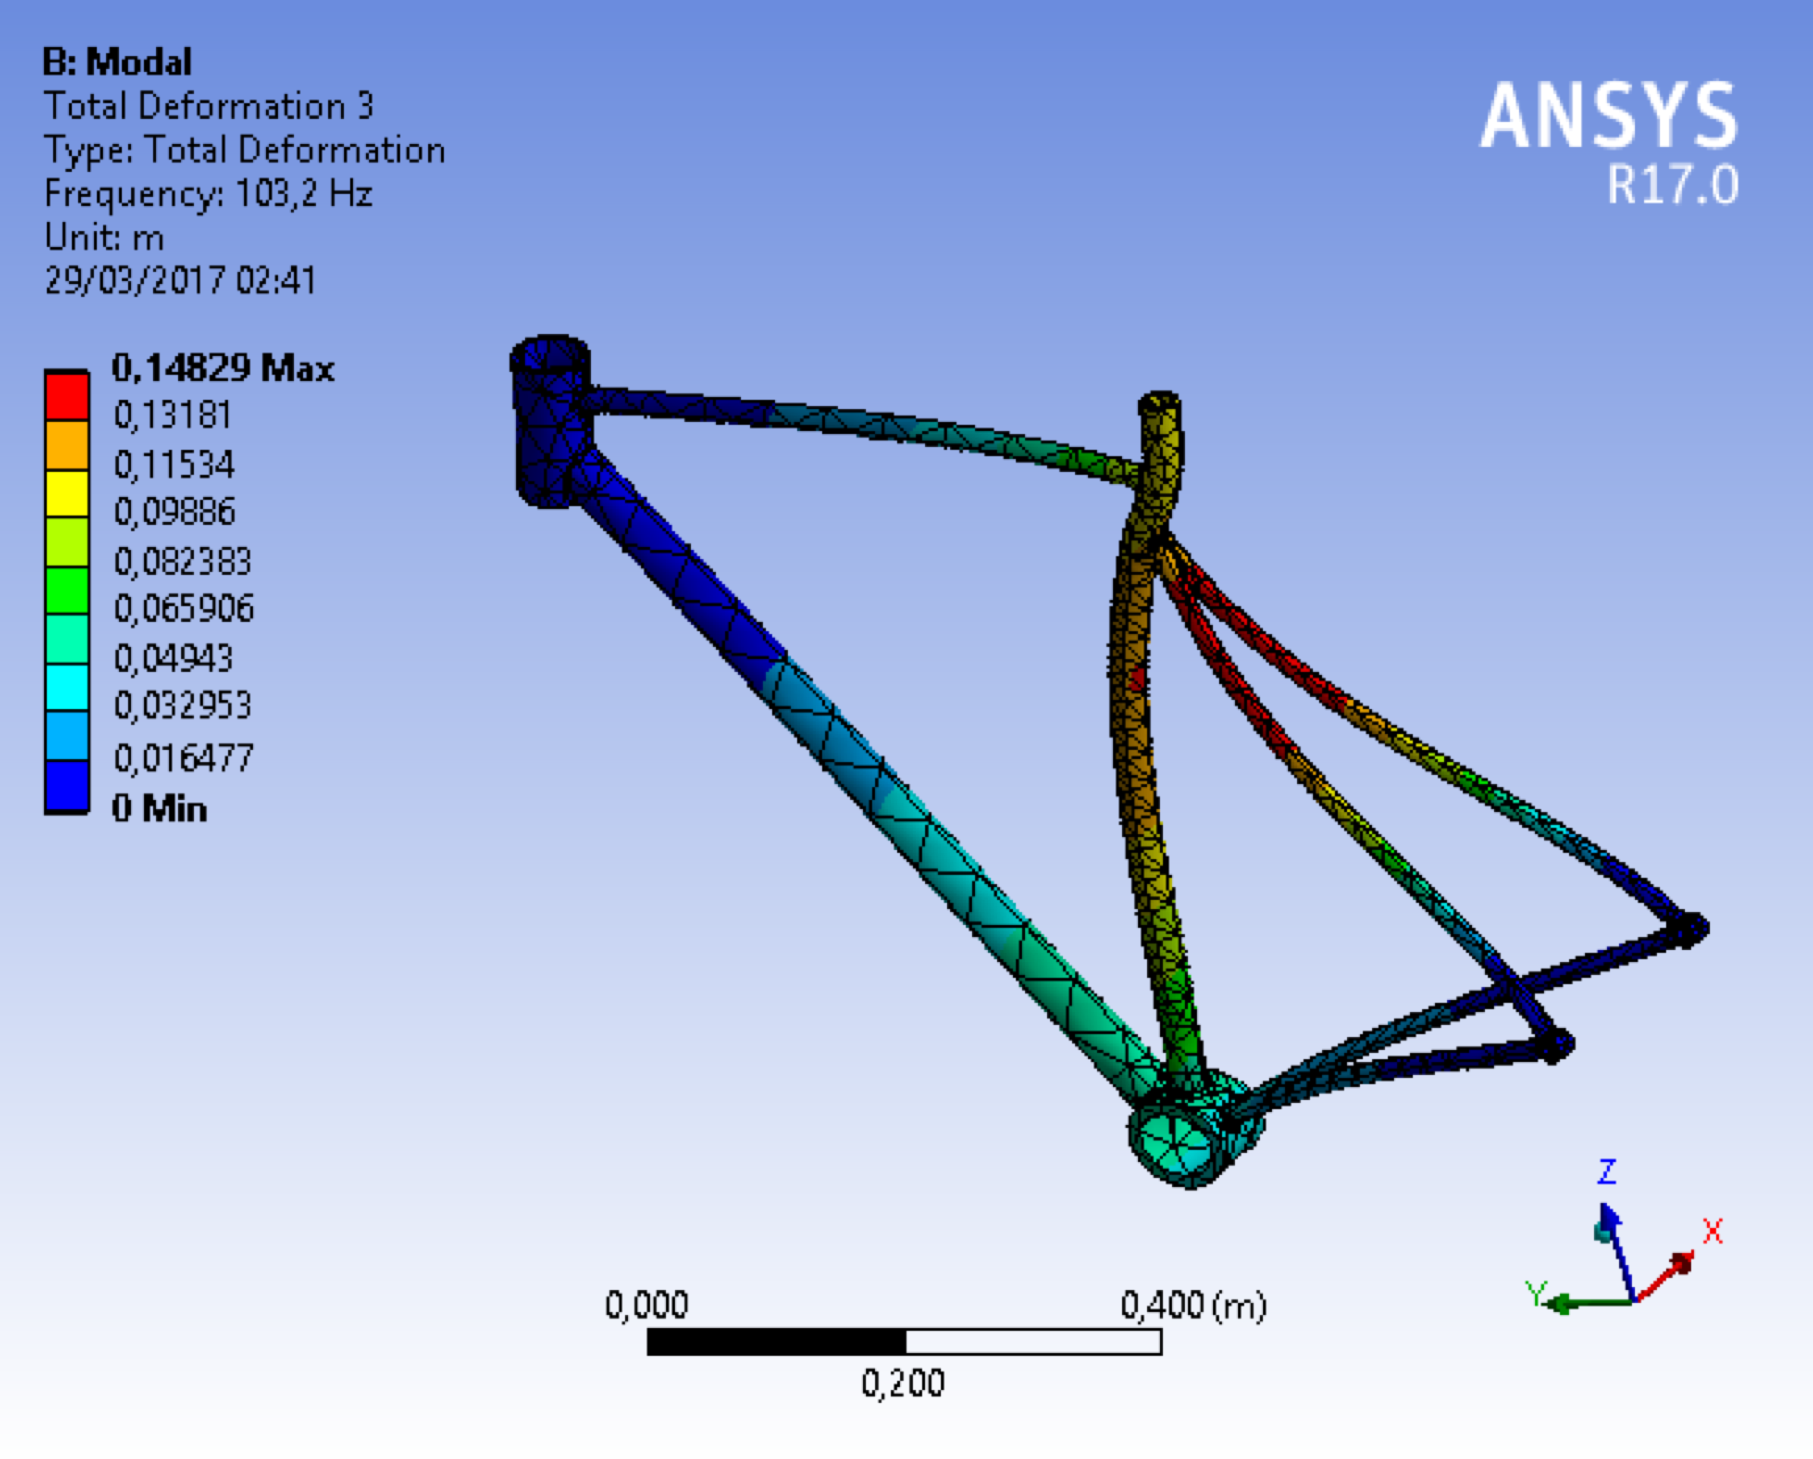
\includegraphics[scale=0.80]{modo_de_vibracao_3.png}
	\caption{Modo de vibracao 3}
	\label{img:modo_de_vibracao3}
	\end{figure}	
	
\graphicspath{{figuras/}}
	\begin{figure}[h!]
	\centering
	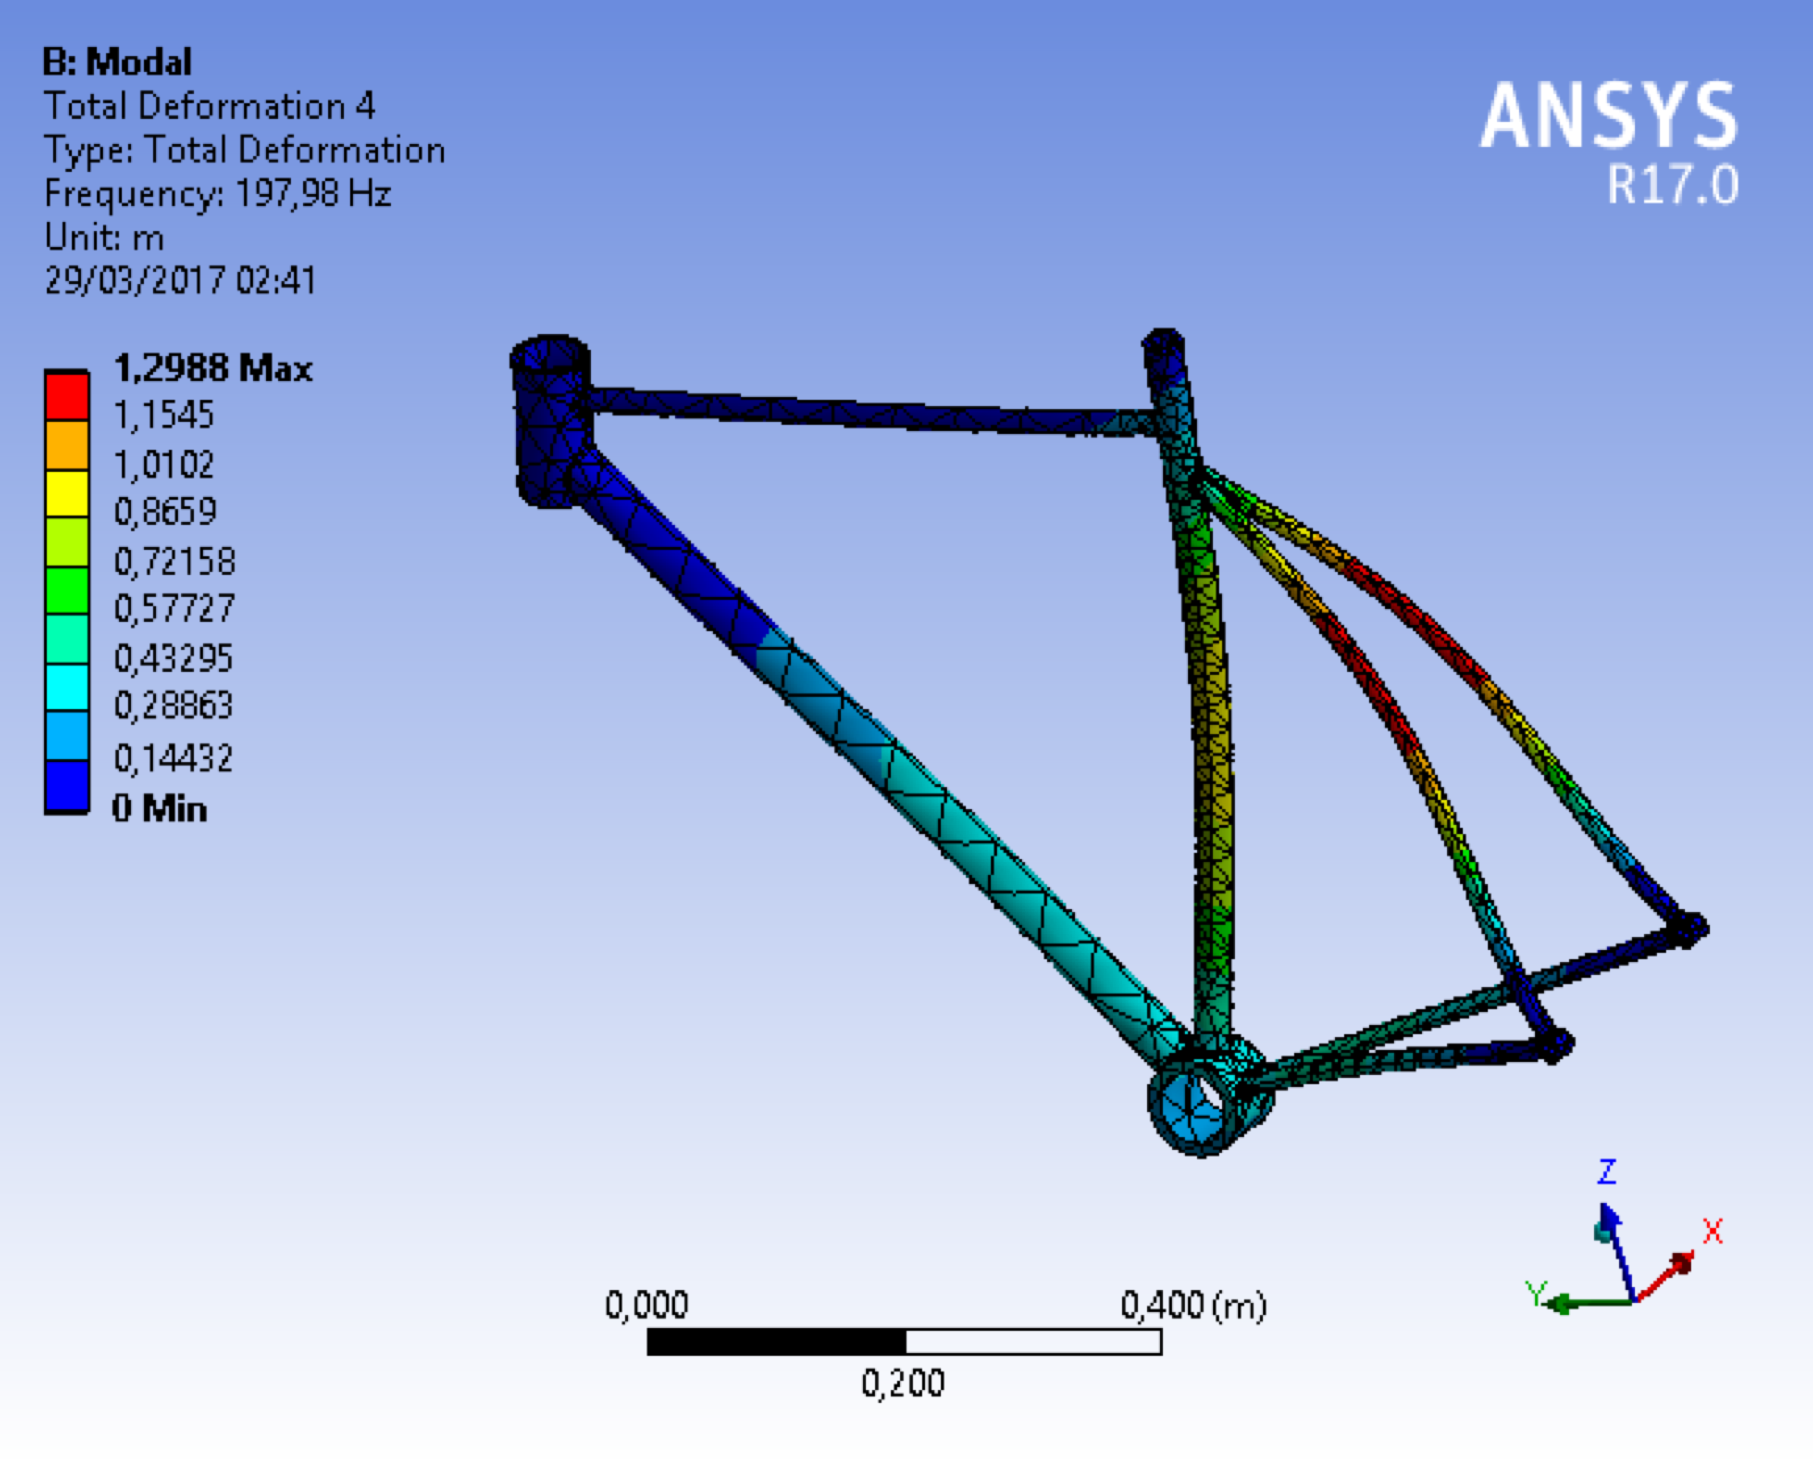
\includegraphics[scale=0.80]{modo_de_vibracao_4.png}
	\caption{Modo de vibracao 4}
	\label{img:modo_de_vibracao4}
	\end{figure}	
	
\graphicspath{{figuras/}}
	\begin{figure}[h!]
	\centering
	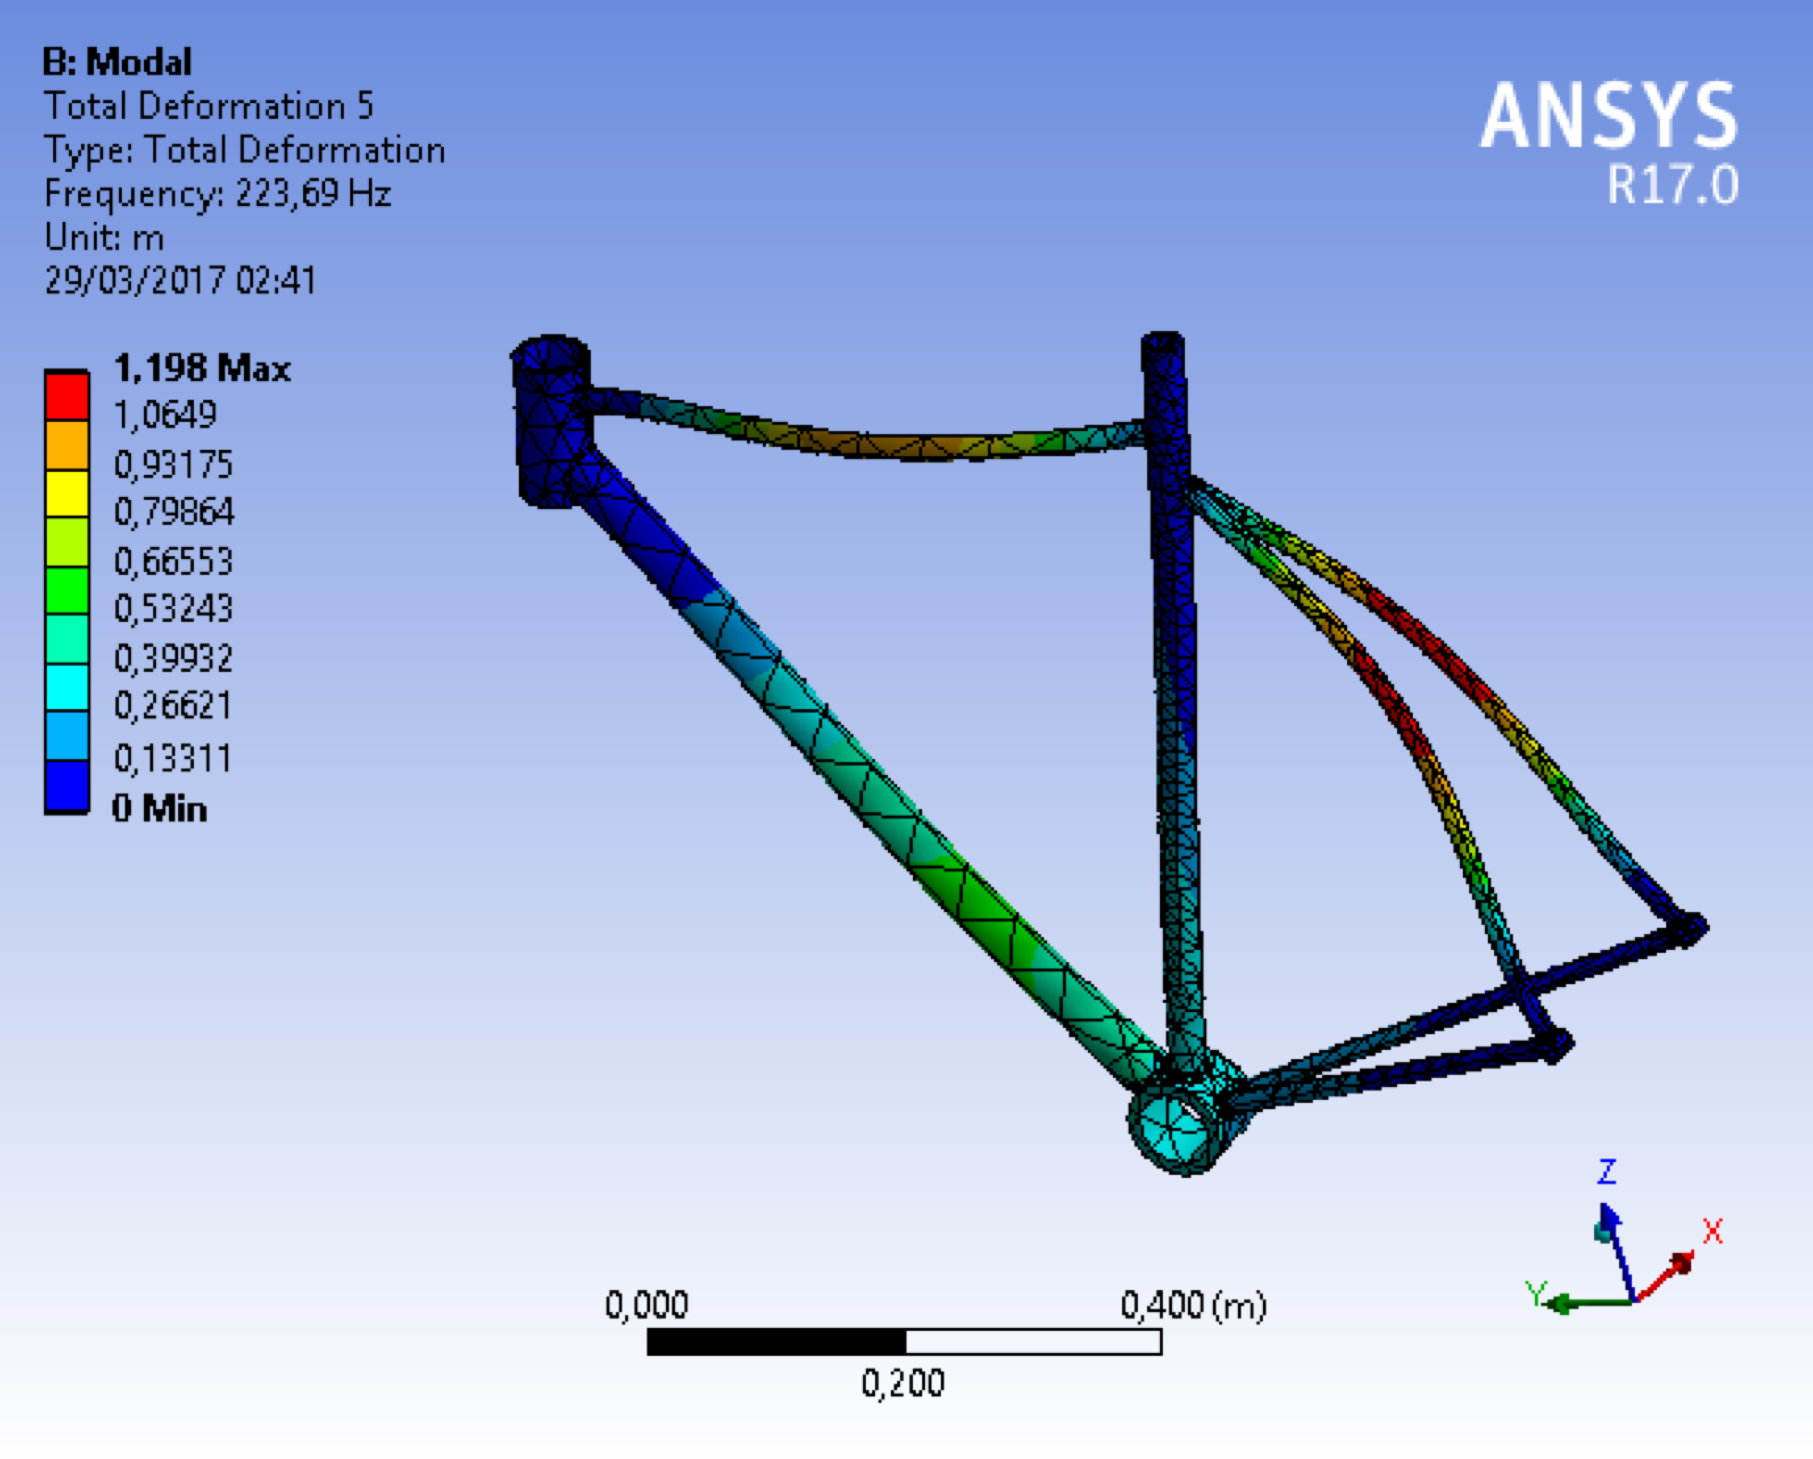
\includegraphics[scale=0.80]{modo_de_vibracao_5.png}
	\caption{Modo de vibracao 5}
	\label{img:modo_de_vibracao5}
	\end{figure}	

\graphicspath{{figuras/}}
	\begin{figure}[h!]
	\centering
	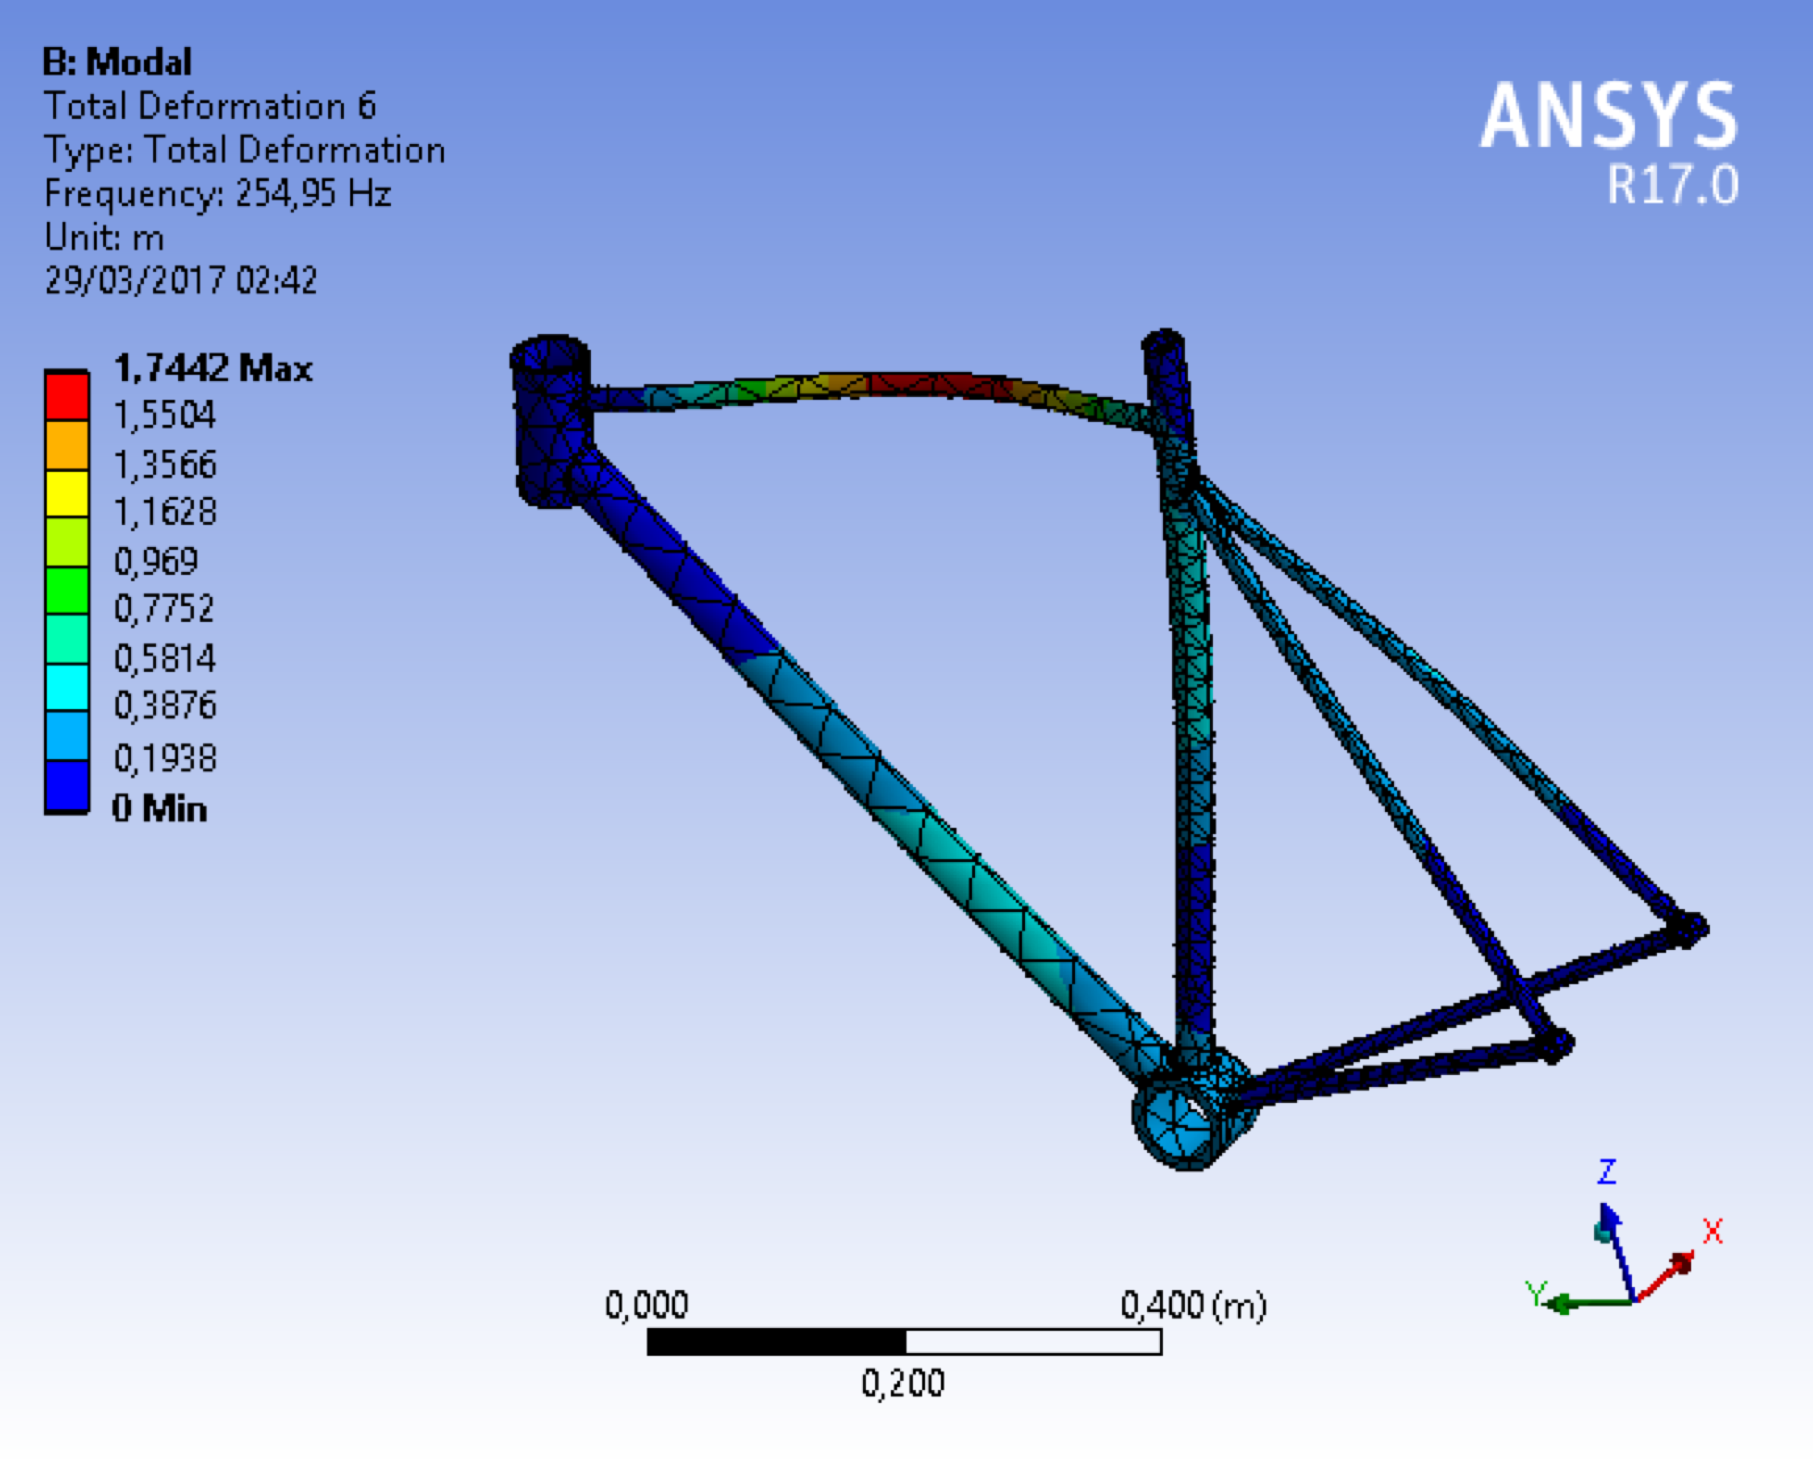
\includegraphics[scale=0.80]{modo_de_vibracao_6.png}
	\caption{Modo de vibracao 6}
	\label{img:modo_de_vibracao 6}
	\end{figure}	



	
	
	
	\subsection{Desafios Técnicos}
	Desafio: Definir uma geometria que comporte todo o sistema sem afetar a ergonomia do ciclista, e que seja capaz de suportar todas as solicitações mecânicas
Alternativa de solução: Alterar a geometria e/ou alterar o material da estrutura.

Desafio: impossibilidade de fabricação do quadro  por escassez de recursos, tempo ou incapacidade técnica.
Alternativa de solução: adquirir um quadro comum no comércio e realizar as adaptações necessárias

  \section{Normas}
  